% Options for packages loaded elsewhere
\PassOptionsToPackage{unicode}{hyperref}
\PassOptionsToPackage{hyphens}{url}
%
\documentclass[
  12pt,
]{article}
\usepackage{amsmath,amssymb}
\usepackage{iftex}
\ifPDFTeX
  \usepackage[T1]{fontenc}
  \usepackage[utf8]{inputenc}
  \usepackage{textcomp} % provide euro and other symbols
\else % if luatex or xetex
  \usepackage{unicode-math} % this also loads fontspec
  \defaultfontfeatures{Scale=MatchLowercase}
  \defaultfontfeatures[\rmfamily]{Ligatures=TeX,Scale=1}
\fi
\usepackage{lmodern}
\ifPDFTeX\else
  % xetex/luatex font selection
\fi
% Use upquote if available, for straight quotes in verbatim environments
\IfFileExists{upquote.sty}{\usepackage{upquote}}{}
\IfFileExists{microtype.sty}{% use microtype if available
  \usepackage[]{microtype}
  \UseMicrotypeSet[protrusion]{basicmath} % disable protrusion for tt fonts
}{}
\makeatletter
\@ifundefined{KOMAClassName}{% if non-KOMA class
  \IfFileExists{parskip.sty}{%
    \usepackage{parskip}
  }{% else
    \setlength{\parindent}{0pt}
    \setlength{\parskip}{6pt plus 2pt minus 1pt}}
}{% if KOMA class
  \KOMAoptions{parskip=half}}
\makeatother
\usepackage{xcolor}
\usepackage[margin=1in]{geometry}
\usepackage{longtable,booktabs,array}
\usepackage{calc} % for calculating minipage widths
% Correct order of tables after \paragraph or \subparagraph
\usepackage{etoolbox}
\makeatletter
\patchcmd\longtable{\par}{\if@noskipsec\mbox{}\fi\par}{}{}
\makeatother
% Allow footnotes in longtable head/foot
\IfFileExists{footnotehyper.sty}{\usepackage{footnotehyper}}{\usepackage{footnote}}
\makesavenoteenv{longtable}
\usepackage{graphicx}
\makeatletter
\def\maxwidth{\ifdim\Gin@nat@width>\linewidth\linewidth\else\Gin@nat@width\fi}
\def\maxheight{\ifdim\Gin@nat@height>\textheight\textheight\else\Gin@nat@height\fi}
\makeatother
% Scale images if necessary, so that they will not overflow the page
% margins by default, and it is still possible to overwrite the defaults
% using explicit options in \includegraphics[width, height, ...]{}
\setkeys{Gin}{width=\maxwidth,height=\maxheight,keepaspectratio}
% Set default figure placement to htbp
\makeatletter
\def\fps@figure{htbp}
\makeatother
\setlength{\emergencystretch}{3em} % prevent overfull lines
\providecommand{\tightlist}{%
  \setlength{\itemsep}{0pt}\setlength{\parskip}{0pt}}
\setcounter{secnumdepth}{5}
\usepackage[OT4]{polski}
\usepackage[utf8]{inputenc}
\usepackage{graphicx}
\usepackage{float}
\usepackage{xcolor}
\usepackage{booktabs}
\usepackage{longtable}
\usepackage{array}
\usepackage{multirow}
\usepackage{wrapfig}
\usepackage{float}
\usepackage{colortbl}
\usepackage{pdflscape}
\usepackage{tabu}
\usepackage{threeparttable}
\usepackage{threeparttablex}
\usepackage[normalem]{ulem}
\usepackage{makecell}
\usepackage{xcolor}
\ifLuaTeX
  \usepackage{selnolig}  % disable illegal ligatures
\fi
\usepackage{bookmark}
\IfFileExists{xurl.sty}{\usepackage{xurl}}{} % add URL line breaks if available
\urlstyle{same}
\hypersetup{
  pdftitle={Sprawozdanie 2},
  pdfauthor={Kacper Szmigielski, 282255 i Mateusz Wizner, 277508},
  hidelinks,
  pdfcreator={LaTeX via pandoc}}

\title{Sprawozdanie 2}
\usepackage{etoolbox}
\makeatletter
\providecommand{\subtitle}[1]{% add subtitle to \maketitle
  \apptocmd{\@title}{\par {\large #1 \par}}{}{}
}
\makeatother
\subtitle{Eksploracja danych}
\author{Kacper Szmigielski, 282255 i Mateusz Wizner, 277508}
\date{2025-04-30}

\begin{document}
\maketitle

{
\setcounter{tocdepth}{3}
\tableofcontents
}
\section{ZADANIE 1 (Dyskretyzacja(przedziałowanie) cech
ciągłych)}\label{zadanie-1-dyskretyzacjaprzedziaux142owanie-cech-ciux105gux142ych}

\subsection{a) Dane: iris (R-pakiet
datasets).}\label{a-dane-iris-r-pakiet-datasets.}

\textbf{3} Pierwsze wiersze z pakietu iris

Zbiór danych zawiera wyniki pomiarów uzyskanych dla \textbf{trzech
gatunków irysów} (tj. setosa, versicolor i virginica) i został
\textbf{udostępniony przez Ronalda Fishera w roku 1936.}

-- \textbf{Pomiary} dotyczą \textbf{długości oraz szerokości} dwóch
różnych części kwiatu-- działki \textbf{kielicha (ang. sepal) oraz
płatka (ang. petal).}

\subsection{b) Wybór cech}\label{b-wybuxf3r-cech}

\textbf{Szukamy cech, których róznice są najbardziej spójne z różnicami
pomiędzy gatunkami.}

\begin{center}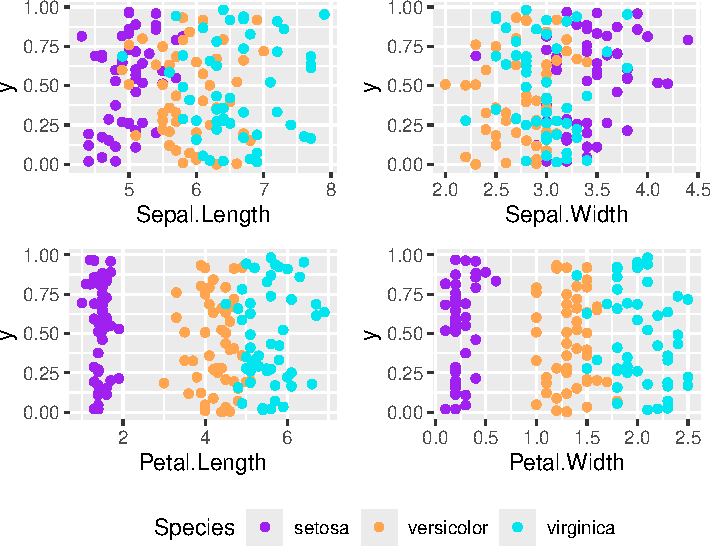
\includegraphics{Sprawozdanie2_files/figure-latex/zad1b1-1} \end{center}

Po przeanalizowaniu scatter-plotów, widać ,że podczas szukania cechy o
najlepszej zdolności dyskretyzacyjnej warto zwrócić uwagę na
\textbf{Petal.Length i Petal.Width}, natomiast jeżeli poszukujemy
kolumny o najgorszej zdolności dyskretyzacyjnej to wybór rozsztrzygamy
spośród \textbf{Sepal.Length i Sepal.Width}

Musimy jednak wybrać \textbf{wartości najlepsze i najgorsze} do
dysktetyzacji, aby to zrobić przeanalizujemy \textbf{box-ploty}.

\begin{center}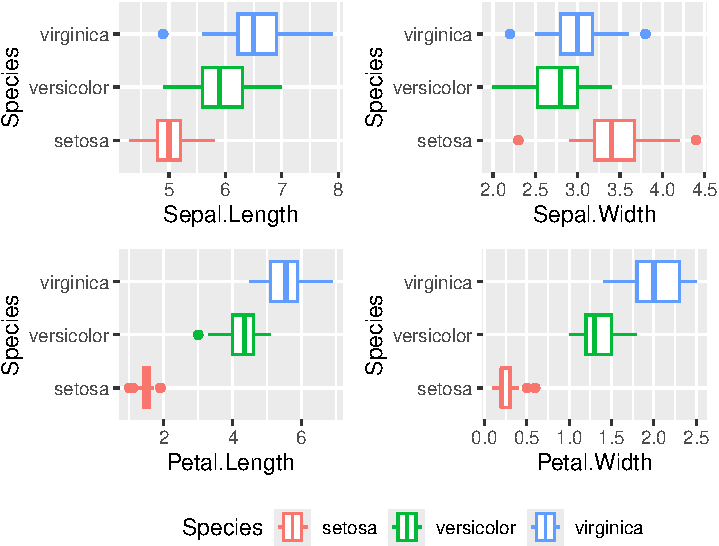
\includegraphics{Sprawozdanie2_files/figure-latex/zad1b2-1} \end{center}

Na ich podstawie możemy uznać, że \textbf{Petal.Width może stanowić
najlepszy wyznacznik gatunku} roślin. \textbf{Najgorszym natomiast jest}
\textbf{Sepal.Width} ponieważ dla \textbf{Petal.Width} gatunki w
najmniejszym stopniu się pokrywają ze względu na tą cechę , a w
\textbf{Sepal.Width} w największym.

\subsection{c) Porównanie nienadzorowanych metod
dyskretyzacji}\label{c-poruxf3wnanie-nienadzorowanych-metod-dyskretyzacji}

\subsubsection{Metoda : Równe
częstości(Frequency)}\label{metoda-ruxf3wne-czux119stoux15bcifrequency}

\paragraph{Dla najlepszej cechy : Petal.Length
(Frequency)}\label{dla-najlepszej-cechy-petal.length-frequency}

\begin{center}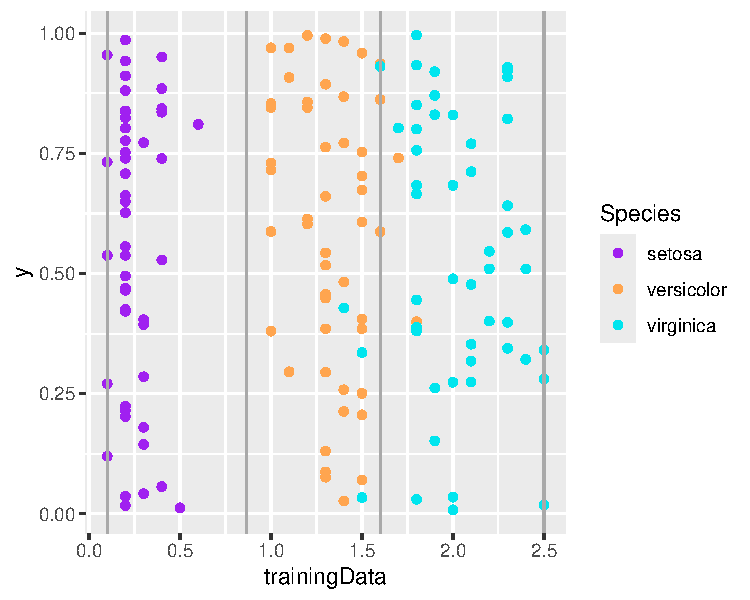
\includegraphics{Sprawozdanie2_files/figure-latex/frequences_najl-1} \end{center}

Widać, że linie uzyskane za pomocną \textbf{Frequency} dość dobrze
rozdzielają nasze dane .

Jeżeli chcemy dokładniej przeanalizować zależność podziału od gatunków,
narysujemy specjalne bar-ploty

\begin{center}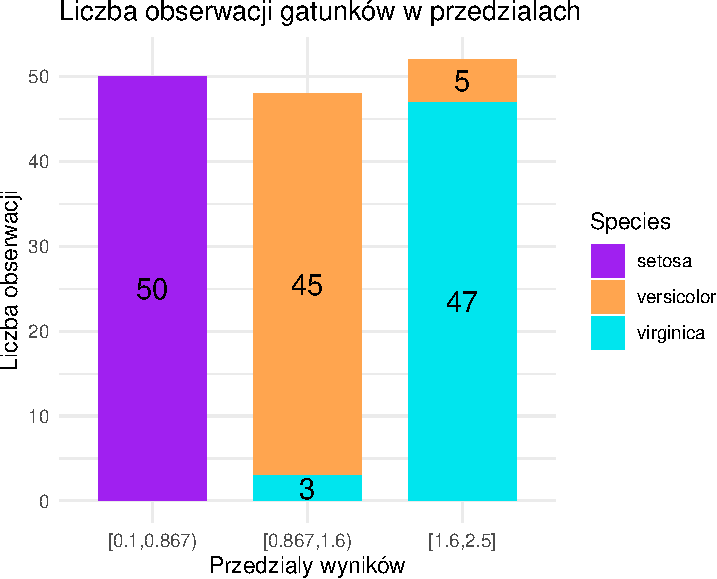
\includegraphics{Sprawozdanie2_files/figure-latex/tabela_kondygnacji_1_najl-1} \end{center}

Świadczą one o tym, że metoda Frequency dla zmiennej
\textbf{Petal.Width} bezproblemowo oddziela gatunek setosa, lecz wśród
pozostałych występuje zjawisko mieszania się (3 virginica
przyporządkowano do versicolor, a 5 versicolor do virginica)

W przypadku tej metody \textbf{zgodność} uzyskanego grupowania z
realnymi wartościami \textbf{wynosi} :

\begin{verbatim}
## [1] 0.9466667
\end{verbatim}

\paragraph{Dla najgorszej cechy : Sepal.Length
(Frequency)}\label{dla-najgorszej-cechy-sepal.length-frequency}

\begin{center}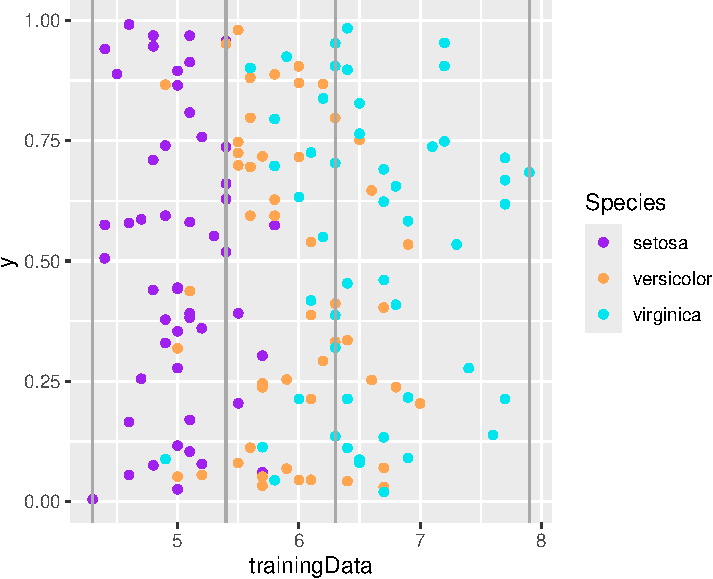
\includegraphics{Sprawozdanie2_files/figure-latex/frequences_najg-1} \end{center}

Scatter-plot wskazuje, że dla Sepal.Length grupowanie może być dość
problematyczne, widać, że obserwacje są dość wymieszane, i trudno będzie
w prosty sposób oddzielić je tak, aby gatunki były prawidłowo
rozłożożone, te sam problem pojawia się w pozostałych metodach grupowań,
dlatego scatter-plot Sepal.Length analizujemy tylko tutaj.

\begin{center}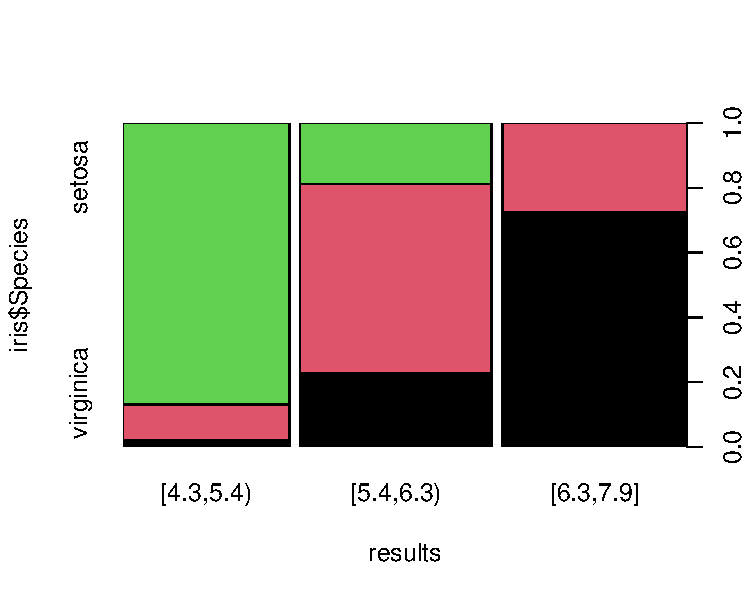
\includegraphics{Sprawozdanie2_files/figure-latex/tabela_kondygnacji_1_najg-1} \end{center}

Na tabeli przyporządkowań widać, problemy metody Frequency, przy
grupowaniu dla zmiennej Sepal.Length, gatunki są dość mocno
przemieszane, brakuje jednolitego podziału.

\begin{verbatim}
## [1] 0.72
\end{verbatim}

Zgodność dla nagjroszej cechy wynosi jedynie ok \textbf{72\%}, co mówi o
znacznym spadku wiarygodności (\textbf{o ok 23 \%}) w porównaniu do
Petal.Width

\subsubsection{Metoda : Równe szerokości
(Interval)}\label{metoda-ruxf3wne-szerokoux15bci-interval}

\paragraph{Dla najlepszej cechy : Petal.Width
(Interval)}\label{dla-najlepszej-cechy-petal.width-interval}

\begin{center}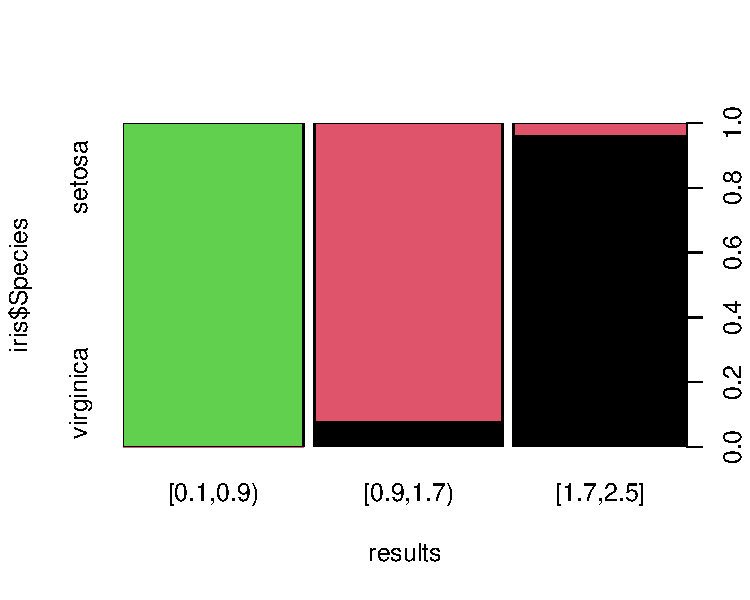
\includegraphics{Sprawozdanie2_files/figure-latex/tabela_kondygnacji_2_najl-1} \end{center}

Po tabeli przyporządkowań widać, że mamy trochę lepsze odróżnienienie
versicolor od virginica

Dla tej metody również mamy \textbf{zgodność na poziomie} :

\begin{verbatim}
## [1] 0.96
\end{verbatim}

Widać lekki wzrost zgodności w porównaniu do poprzedniej metody
(\textbf{o ok 1\%})

\paragraph{Dla najgorszej cechy ; Sepal.Length
(Interval)}\label{dla-najgorszej-cechy-sepal.length-interval}

\begin{center}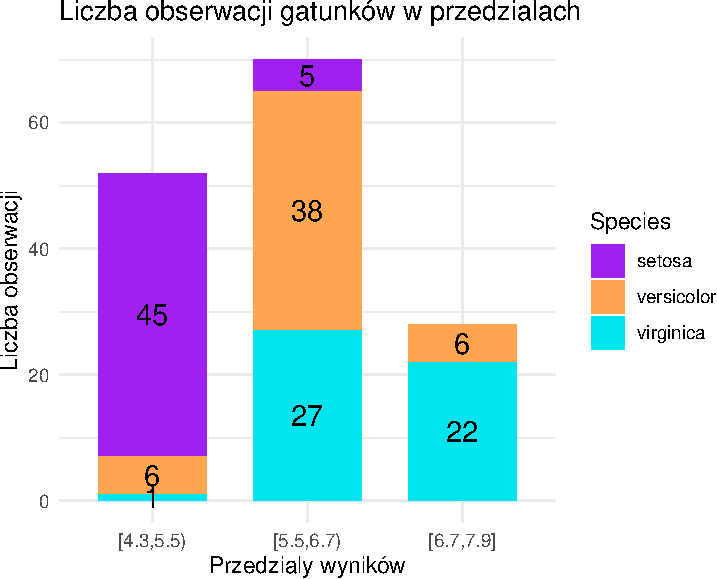
\includegraphics{Sprawozdanie2_files/figure-latex/tabela_kondygnacji_2_najg-1} \end{center}

Dla tabeli zgodności widać, że metoda w zły sposób rozdziela przypadki.
Bardzo duża ich ilość znajduje się w środkowym przedziale, więc nie jest
to dobry podział gatunkowy

Metoda ta, dla najgorszej cechy dyskretyzuje ze zgodnością :

\begin{verbatim}
## [1] 0.5729167
\end{verbatim}

Czyli w porównaniu do metody Frequency mamy \textbf{spadek} aż \textbf{o
ok 16\%}

\subsubsection{Metoda : k najbliższych sąsiadów
(K-means)}\label{metoda-k-najbliux17cszych-sux105siaduxf3w-k-means}

\paragraph{Dla najlepszej cechy : Petal.Width
(K-means)}\label{dla-najlepszej-cechy-petal.width-k-means}

\begin{center}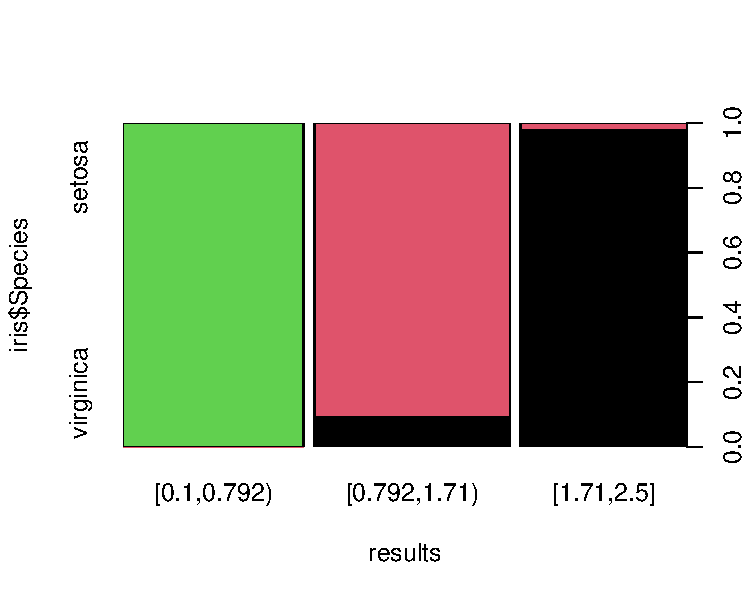
\includegraphics{Sprawozdanie2_files/figure-latex/tabela_kondygnacji_3_najl-1} \end{center}

Analogiczny podział jak w poprzedniej metodzie

Zgodność na poziomie :

\begin{verbatim}
## [1] 0.96
\end{verbatim}

Lepsza \textbf{o ok 3\%} od ubiegłej metody

\paragraph{Dla najgorszej cechy : Sepal.Length
(K-means)}\label{dla-najgorszej-cechy-sepal.length-k-means}

\begin{center}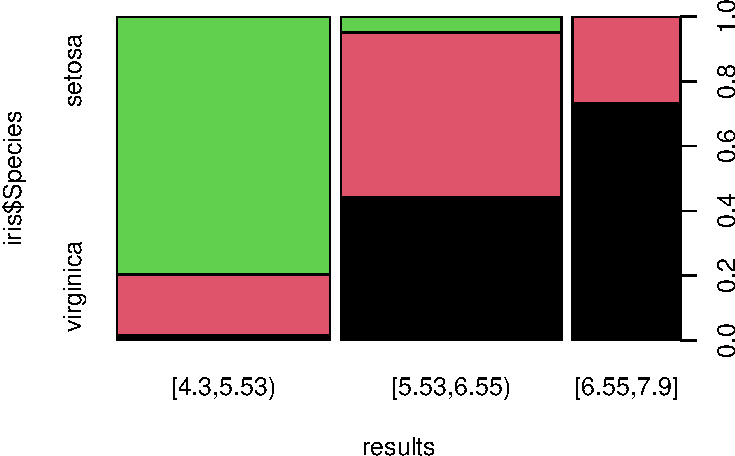
\includegraphics{Sprawozdanie2_files/figure-latex/tabela_kondygnacji_3_najg-1} \end{center}

Bardziej równomierne rozłożenie niż w metodzie poprzedniej, lecz nie
jest wciąż dobre pod względem gatunkowym.

Dla najgorszej cechy mamy zgodność :

\begin{verbatim}
## [1] 0.5589744
\end{verbatim}

W tym przypadku jest ona \textbf{na poziome metody Frequency (gorsza o
1)}

\subsubsection{Dyskretyzacja z przedziałami zadanymi przez urzytkownika
(fixed)}\label{dyskretyzacja-z-przedziaux142ami-zadanymi-przez-urzytkownika-fixed}

\paragraph{Dla najlepszej cechy : Petal.Width
(fixed)}\label{dla-najlepszej-cechy-petal.width-fixed}

\begin{center}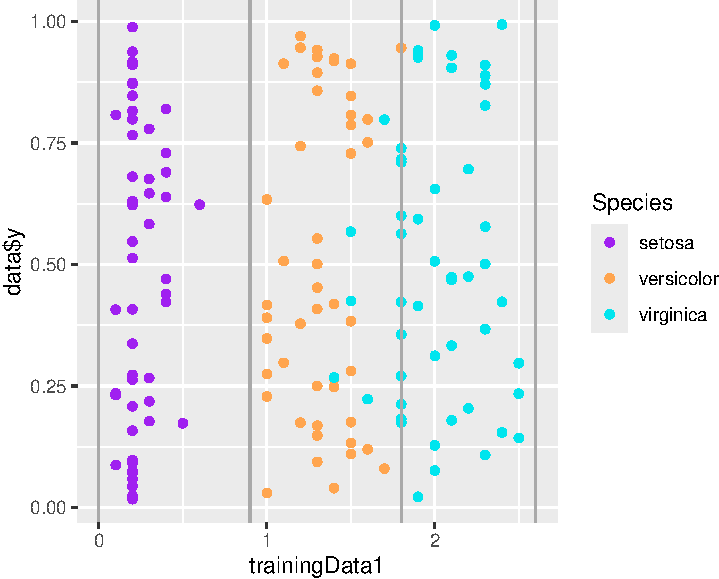
\includegraphics{Sprawozdanie2_files/figure-latex/givenRanges_najl-1} \end{center}

Na wykresie mamy zaznaczone też końce przedziałów, co jest potrzebne
podczas wizualizacji przedziałów zadanych przez użytkownika.

\begin{center}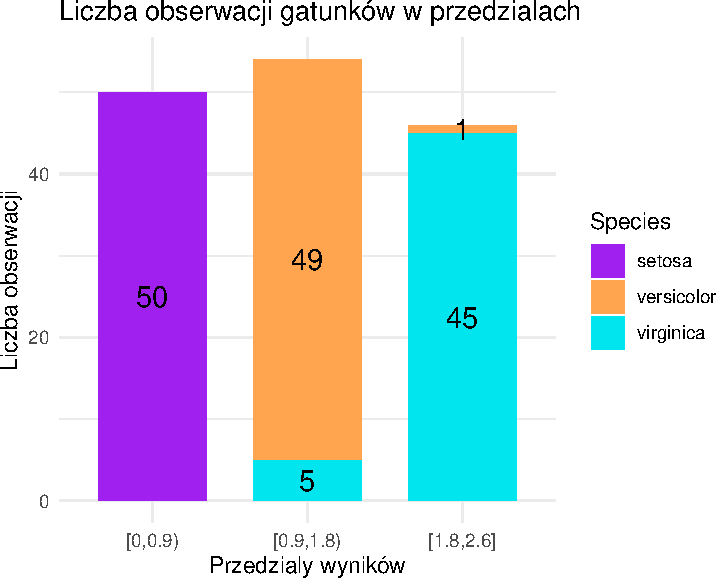
\includegraphics{Sprawozdanie2_files/figure-latex/tabela_kondygnacji_4_najl-1} \end{center}

Mamy najmniejsze rozmieszanie virignica i versicolor. Tylko 1 versicolor
została źle przyporządkowana w porównaniu do aż 5 virginic.

Zgodność na poziome poprzednich dwóch metod, wynosi :

\begin{verbatim}
## [1] 0.96
\end{verbatim}

\paragraph{Dla najgorszej cechy : Sepal.Length
(fixed)}\label{dla-najgorszej-cechy-sepal.length-fixed}

\begin{center}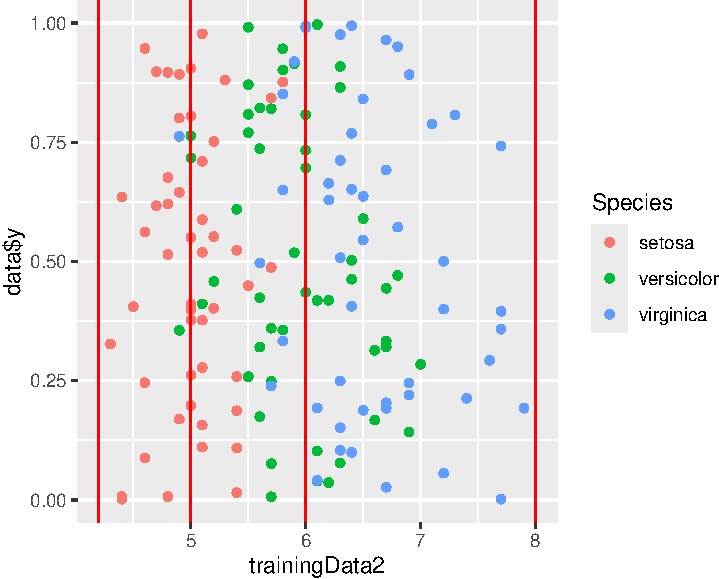
\includegraphics{Sprawozdanie2_files/figure-latex/givenRanges_najg-1} \end{center}

\begin{center}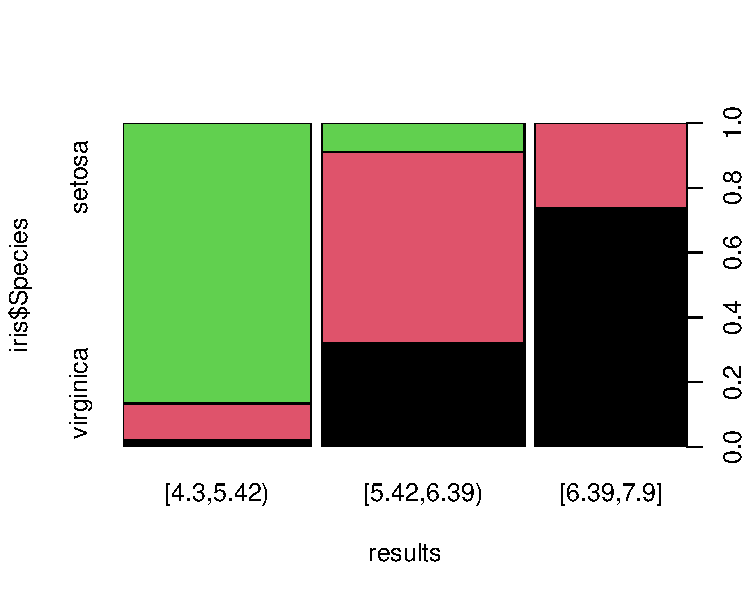
\includegraphics{Sprawozdanie2_files/figure-latex/tabela_kondygnacji_4_najg-1} \end{center}

Równomierny rozkład między pierwszymi dwoma przedziałami ale dalej
nierozróżnialne na postawie tej metody, więc nie powinniśmy używać jej
do dyskretyzacji.

Dla cechy o najgorszej zdolności dyskretyzacynej:

\begin{verbatim}
## [1] 0.72
\end{verbatim}

\subsection{Wnioski :}\label{wnioski}

\textbf{Porównamy teraz} zgodności procentowe \textbf{wyników}, dla
\textbf{poszczególnych algorytmów}

\begin{longtable}[]{@{}lrrrr@{}}
\toprule\noalign{}
& frequency & interval & cluster & fixed \\
\midrule\noalign{}
\endhead
\bottomrule\noalign{}
\endlastfoot
Petal.Width & 0.9466667 & 0.9600000 & 0.9600000 & 0.96 \\
Sepal.Length & 0.7200000 & 0.5729167 & 0.5589744 & 0.72 \\
\end{longtable}

Na podstawie tabeli \textbf{przyporządkowań} dla cech najgorszych i
najlepszych pod względem dyskretyzacji możemy wnioskować, że dla
obecnych danych \textbf{najlepszym} algorytmem jest
\textbf{frequency(częstość)}. Odznacza się dobrym przyporządkowaniem dla
\textbf{Petal.Width} i najlepszym dla \textbf{Sepal.Length}

\section{ZADANIE 2 (Analizaskładowych głównych (Principal Component
Analysis
(PCA)))}\label{zadanie-2-analizaskux142adowych-gux142uxf3wnych-principal-component-analysis-pca}

\subsection{a) Przygotowanie i opis
danych}\label{a-przygotowanie-i-opis-danych}

\textbf{Podstawowe} informacje nt. danych \textbf{uaScoresDataFrame}

\begin{longtable}[]{@{}lr@{}}
\toprule\noalign{}
\endhead
\bottomrule\noalign{}
\endlastfoot
rows & 266 \\
columns & 21 \\
discrete\_columns & 3 \\
continuous\_columns & 18 \\
all\_missing\_columns & 0 \\
total\_missing\_values & 0 \\
complete\_rows & 266 \\
total\_observations & 5586 \\
memory\_usage & 73496 \\
\end{longtable}

Dane zawierają informacje o \textbf{266} miastach, obejmujące
\textbf{21} cech, z których \textbf{18} to zmienne ciągłe, a \textbf{3}
dyskretne. Zbiór jest \textbf{kompletny}, bez brakujących wartości, co
oznacza pełne \textbf{5586} obserwacji.

\textbf{Typy danych} w zbiorze

\begin{center}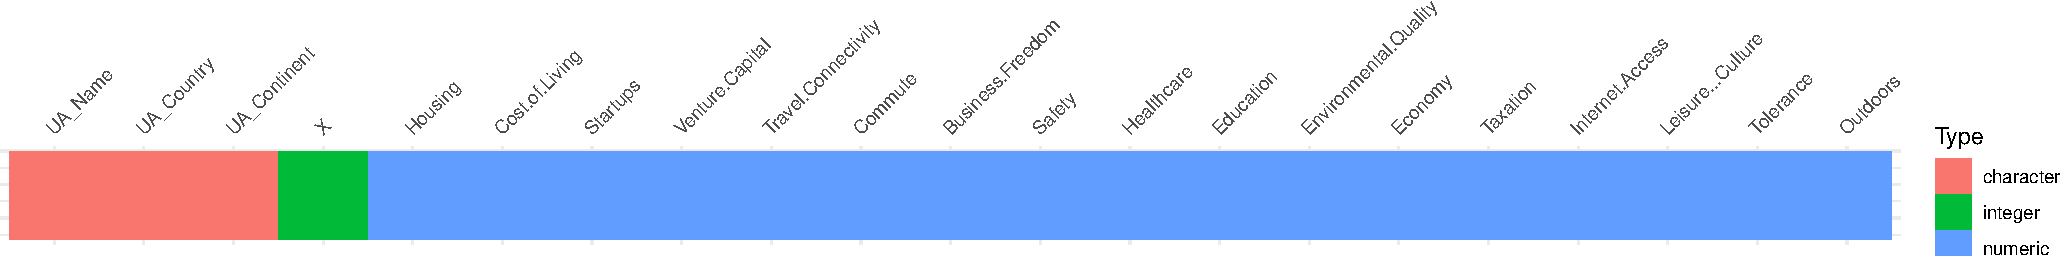
\includegraphics{Sprawozdanie2_files/figure-latex/typy_danych-1} \end{center}

\textbf{Tabela poniżej} przedstawia \textbf{pięć} przykładowych wierszy
danych.

\begin{table}[!h]
\centering
\resizebox{\ifdim\width>\linewidth\linewidth\else\width\fi}{!}{
\begin{tabular}{rlllrrrrrr}
\toprule
X & UA\_Name & UA\_Country & UA\_Continent & Housing & Cost.of.Living & Startups & Venture.Capital & Travel.Connectivity & Commute\\
\midrule
\cellcolor{gray!10}{0} & \cellcolor{gray!10}{Aarhus} & \cellcolor{gray!10}{Denmark} & \cellcolor{gray!10}{Europe} & \cellcolor{gray!10}{6.132} & \cellcolor{gray!10}{4.015} & \cellcolor{gray!10}{2.827} & \cellcolor{gray!10}{2.512} & \cellcolor{gray!10}{3.536} & \cellcolor{gray!10}{6.312}\\
1 & Adelaide & Australia & Oceania & 6.310 & 4.692 & 3.136 & 2.640 & 1.777 & 5.336\\
\cellcolor{gray!10}{2} & \cellcolor{gray!10}{Albuquerque} & \cellcolor{gray!10}{New Mexico} & \cellcolor{gray!10}{North America} & \cellcolor{gray!10}{7.262} & \cellcolor{gray!10}{6.059} & \cellcolor{gray!10}{3.772} & \cellcolor{gray!10}{1.493} & \cellcolor{gray!10}{1.456} & \cellcolor{gray!10}{5.056}\\
3 & Almaty & Kazakhstan & Asia & 9.282 & 9.333 & 2.458 & 0.000 & 4.592 & 5.871\\
\cellcolor{gray!10}{4} & \cellcolor{gray!10}{Amsterdam} & \cellcolor{gray!10}{Netherlands} & \cellcolor{gray!10}{Europe} & \cellcolor{gray!10}{3.053} & \cellcolor{gray!10}{3.824} & \cellcolor{gray!10}{7.972} & \cellcolor{gray!10}{6.107} & \cellcolor{gray!10}{8.325} & \cellcolor{gray!10}{6.118}\\
\addlinespace
5 & Anchorage & Alaska & North America & 5.434 & 3.141 & 2.795 & 0.000 & 1.738 & 4.715\\
\bottomrule
\end{tabular}}
\end{table}

\begin{table}[!h]
\centering
\resizebox{\ifdim\width>\linewidth\linewidth\else\width\fi}{!}{
\begin{tabular}{rrrrrrrrrrrr}
\toprule
X & Business.Freedom & Safety & Healthcare & Education & Environmental.Quality & Economy & Taxation & Internet.Access & Leisure...Culture & Tolerance & Outdoors\\
\midrule
\cellcolor{gray!10}{0} & \cellcolor{gray!10}{9.940} & \cellcolor{gray!10}{9.617} & \cellcolor{gray!10}{8.704} & \cellcolor{gray!10}{5.367} & \cellcolor{gray!10}{7.633} & \cellcolor{gray!10}{4.887} & \cellcolor{gray!10}{5.068} & \cellcolor{gray!10}{8.373} & \cellcolor{gray!10}{3.187} & \cellcolor{gray!10}{9.739} & \cellcolor{gray!10}{4.130}\\
1 & 9.400 & 7.926 & 7.937 & 5.142 & 8.331 & 6.070 & 4.588 & 4.341 & 4.328 & 7.822 & 5.531\\
\cellcolor{gray!10}{2} & \cellcolor{gray!10}{8.671} & \cellcolor{gray!10}{1.343} & \cellcolor{gray!10}{6.430} & \cellcolor{gray!10}{4.152} & \cellcolor{gray!10}{7.319} & \cellcolor{gray!10}{6.514} & \cellcolor{gray!10}{4.346} & \cellcolor{gray!10}{5.396} & \cellcolor{gray!10}{4.890} & \cellcolor{gray!10}{7.028} & \cellcolor{gray!10}{3.515}\\
3 & 5.568 & 7.309 & 4.546 & 2.283 & 3.857 & 5.269 & 8.522 & 2.886 & 2.937 & 6.540 & 5.500\\
\cellcolor{gray!10}{4} & \cellcolor{gray!10}{8.837} & \cellcolor{gray!10}{8.504} & \cellcolor{gray!10}{7.907} & \cellcolor{gray!10}{6.180} & \cellcolor{gray!10}{7.597} & \cellcolor{gray!10}{5.053} & \cellcolor{gray!10}{4.955} & \cellcolor{gray!10}{4.523} & \cellcolor{gray!10}{8.874} & \cellcolor{gray!10}{8.368} & \cellcolor{gray!10}{5.307}\\
\addlinespace
5 & 8.671 & 3.470 & 6.060 & 3.624 & 9.272 & 6.514 & 4.772 & 4.964 & 3.266 & 7.093 & 5.358\\
\bottomrule
\end{tabular}}
\end{table}

\begin{center}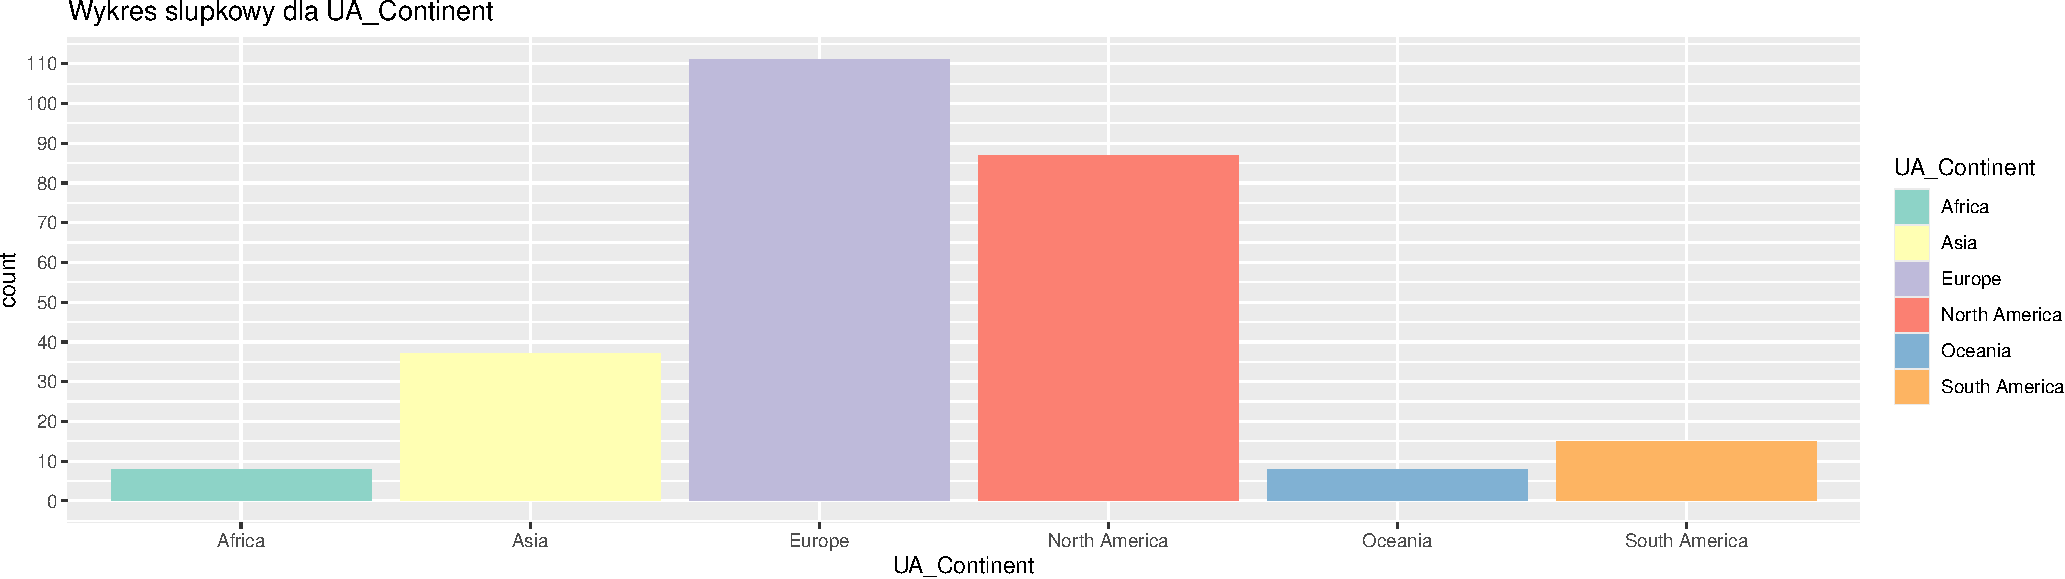
\includegraphics{Sprawozdanie2_files/figure-latex/wykresy_jakosciowe-1} \end{center}

\begin{center}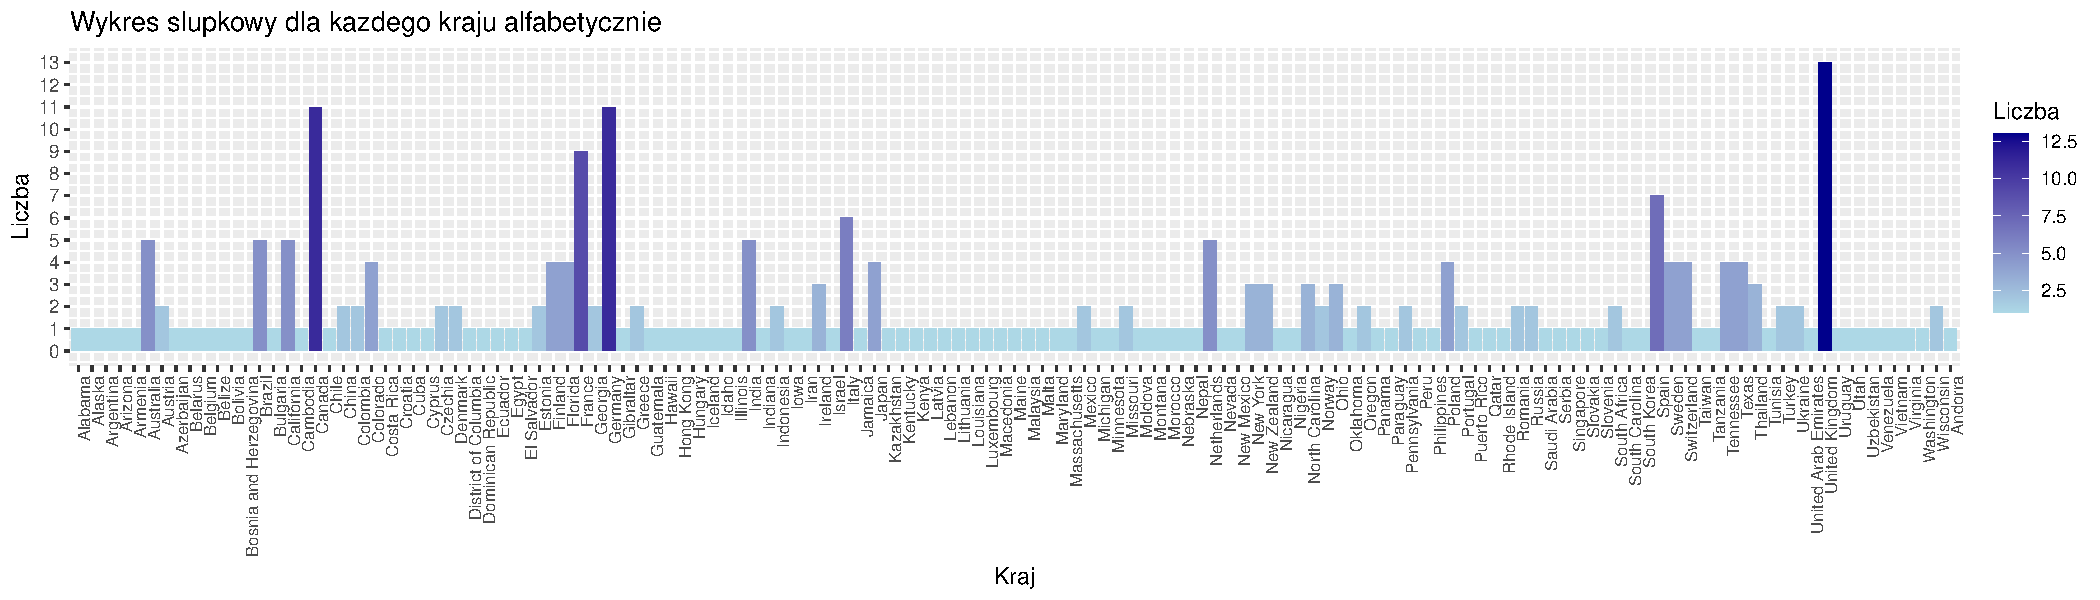
\includegraphics{Sprawozdanie2_files/figure-latex/wykresy_country_ilosc_rekordow-1} \end{center}

\begin{center}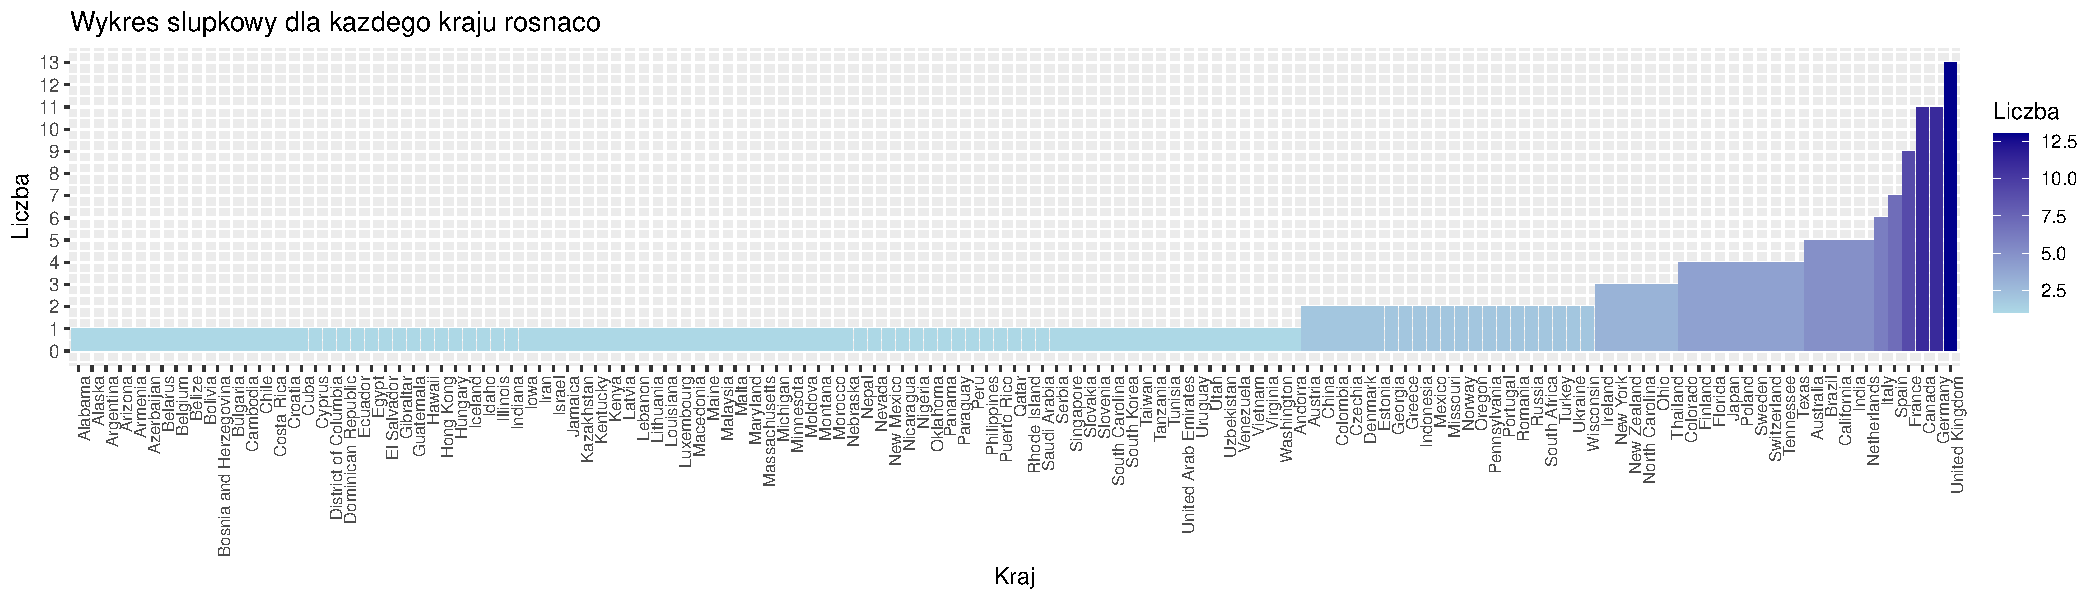
\includegraphics{Sprawozdanie2_files/figure-latex/wykresy_country_ilosc_rekordow-2} \end{center}

\textbf{Analiza wykresów} wskazuje, że \textbf{większość rekordów}
pochodzi z \textbf{krajów rozwiniętych}, głównie z \textbf{Europy} i
\textbf{Ameryki Północnej}.

\begin{center}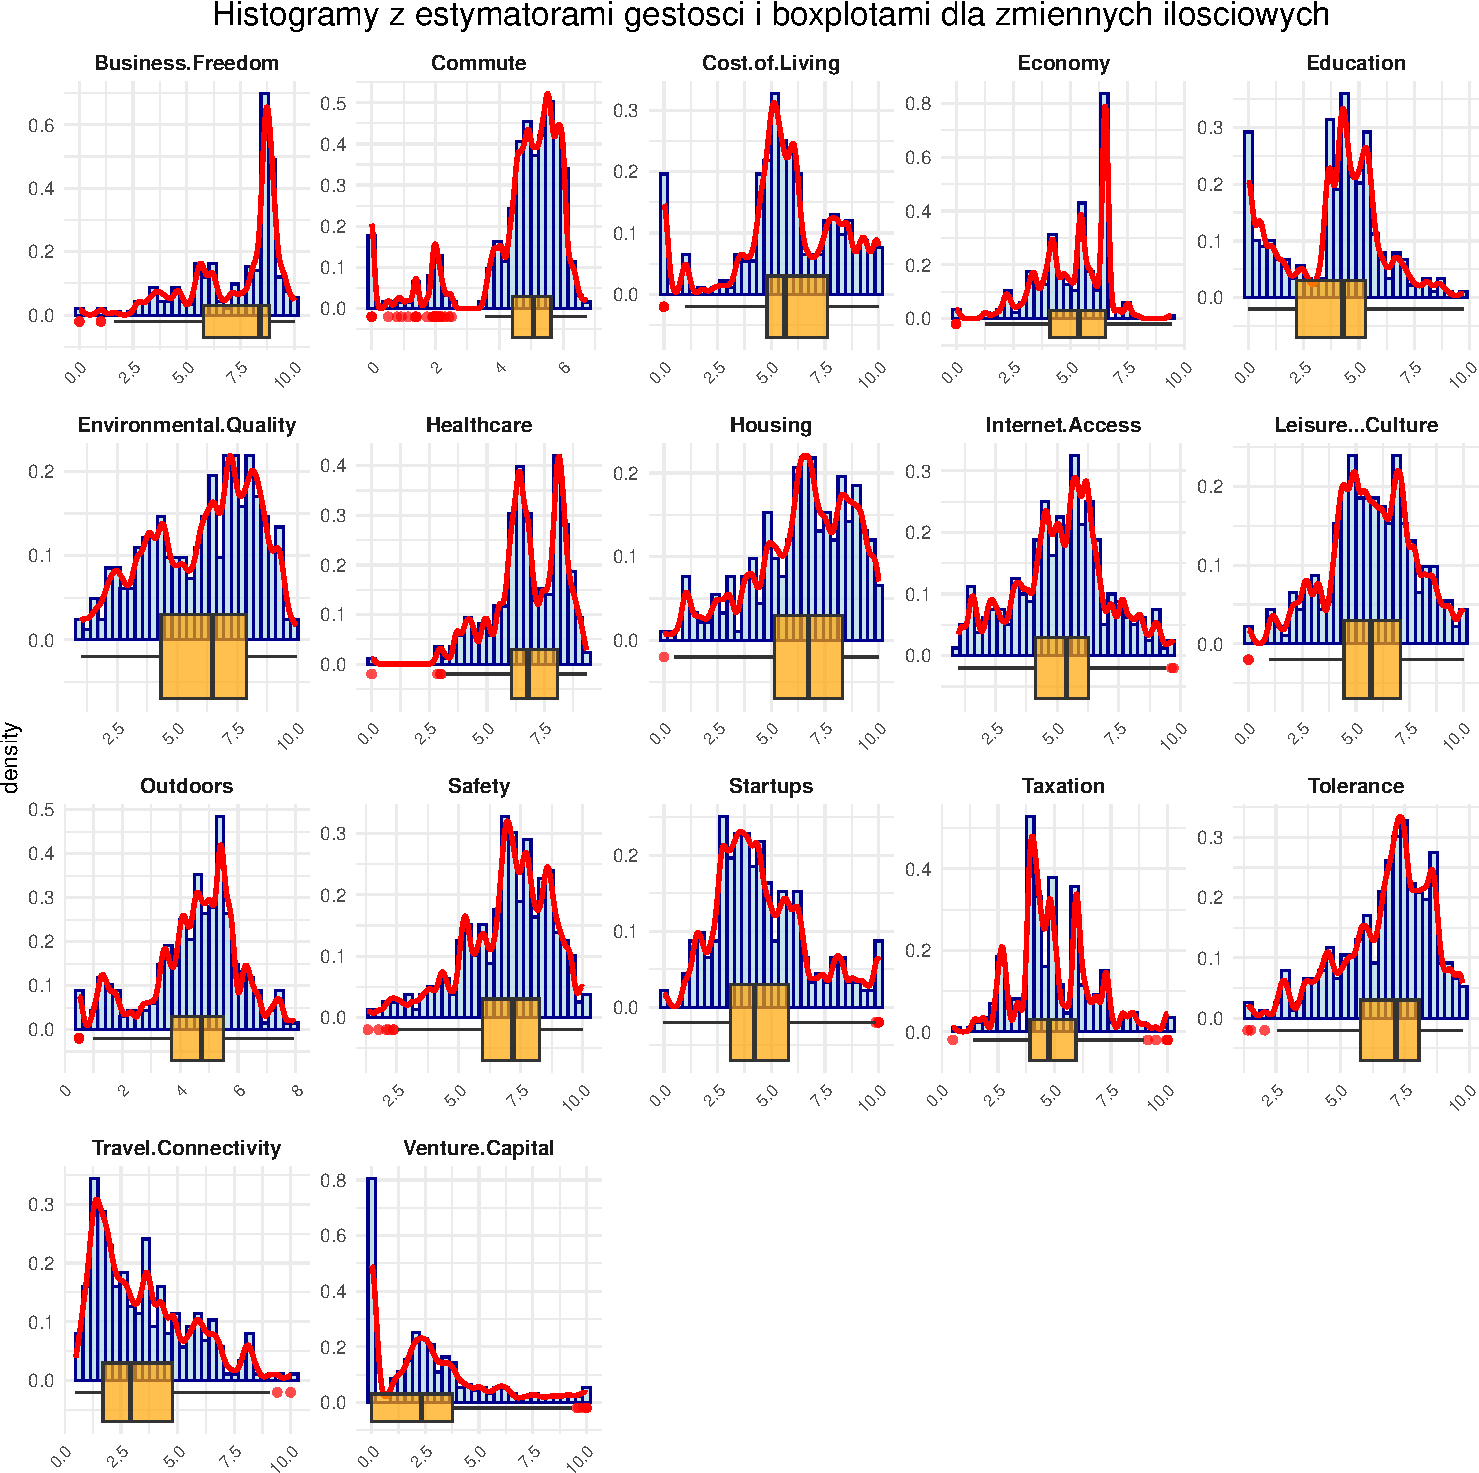
\includegraphics{Sprawozdanie2_files/figure-latex/histogramy_ilosciowe1-1} \end{center}

\begin{center}\rule{0.5\linewidth}{0.5pt}\end{center}

\textbf{Wolność biznesowa (Business.Freedom):}\\
Większość miast zapewnia dobre warunki dla biznesu (szczyt ok. 8.5),
niewiele wypada słabo (\textless5).

\textbf{Dojazdy (Commute):}\\
Większość miast cechuje się przeciętnym/słabym poziomem skomunikowania
(4--6).

\textbf{Koszty życia (Cost.of.Living):}\\
Podział na miasta średnio drogie (szczyt 5--6) i drogie (7--8).

\textbf{Gospodarka (Economy):}\\
Większość miast ma silną gospodarkę (szczyt 8--9), niewiele słabych
(\textless5).

\textbf{Edukacja (Education):}\\
Wyraźny podział -- bardzo niski (0--2) i przeciętny (4--6) poziom
edukacji.

\textbf{Jakość środowiska (Environmental.Quality):}\\
Większość miast z dobrą jakością środowiska (6--8).

\textbf{Opieka zdrowotna (Healthcare):}\\
Podział na miasta z dobrą (8-9) i przeciętną (5--6) opieką, mało słabych

\textbf{Mieszkalnictwo (Housing):}\\
Dominują przeciętne warunki (5--6), część z bardzo dobrymi (8--9).

\textbf{Dostęp do internetu (Internet.Access):}\\
Powszechnie przeciętny dostęp (5--7)

\textbf{Kultura i rozrywka (Leisure.\&.Culture):}\\
Przyzwoity poziom w większości miast (5--7).

\textbf{Aktywności na świeżym powietrzu (Outdoors):}\\
Głównie średni poziom (4 - 6)

\textbf{Bezpieczeństwo (Safety):}\\
Większość miast jest bezpieczna (6-9)

\textbf{Startupy (Startups):}\\
Większość miast przeciętna (4--5), mniejsza grupa z bardzo dobrymi
warunkami (9--10).

\textbf{Podatki (Taxation):}\\
Większość miast z umiarkowanymi lub wysokimi podatkami (4--5).

\textbf{Tolerancja (Tolerance):}\\
Dominują wysokie oceny (7--8), bardzo mało niskich (\textless4).

\textbf{Połączenia komunikacyjne (Travel.Connectivity):}\\
Większość miast ze słabymi połączeniami (2--3), tylko nieliczne dobre
(6--7).

\textbf{Kapitał venture (Venture.Capital):}\\
Dostęp bardzo ograniczony -- większość miast w przedziale 1--2,
nieliczne wyjątki.

\begin{center}\rule{0.5\linewidth}{0.5pt}\end{center}

\begin{center}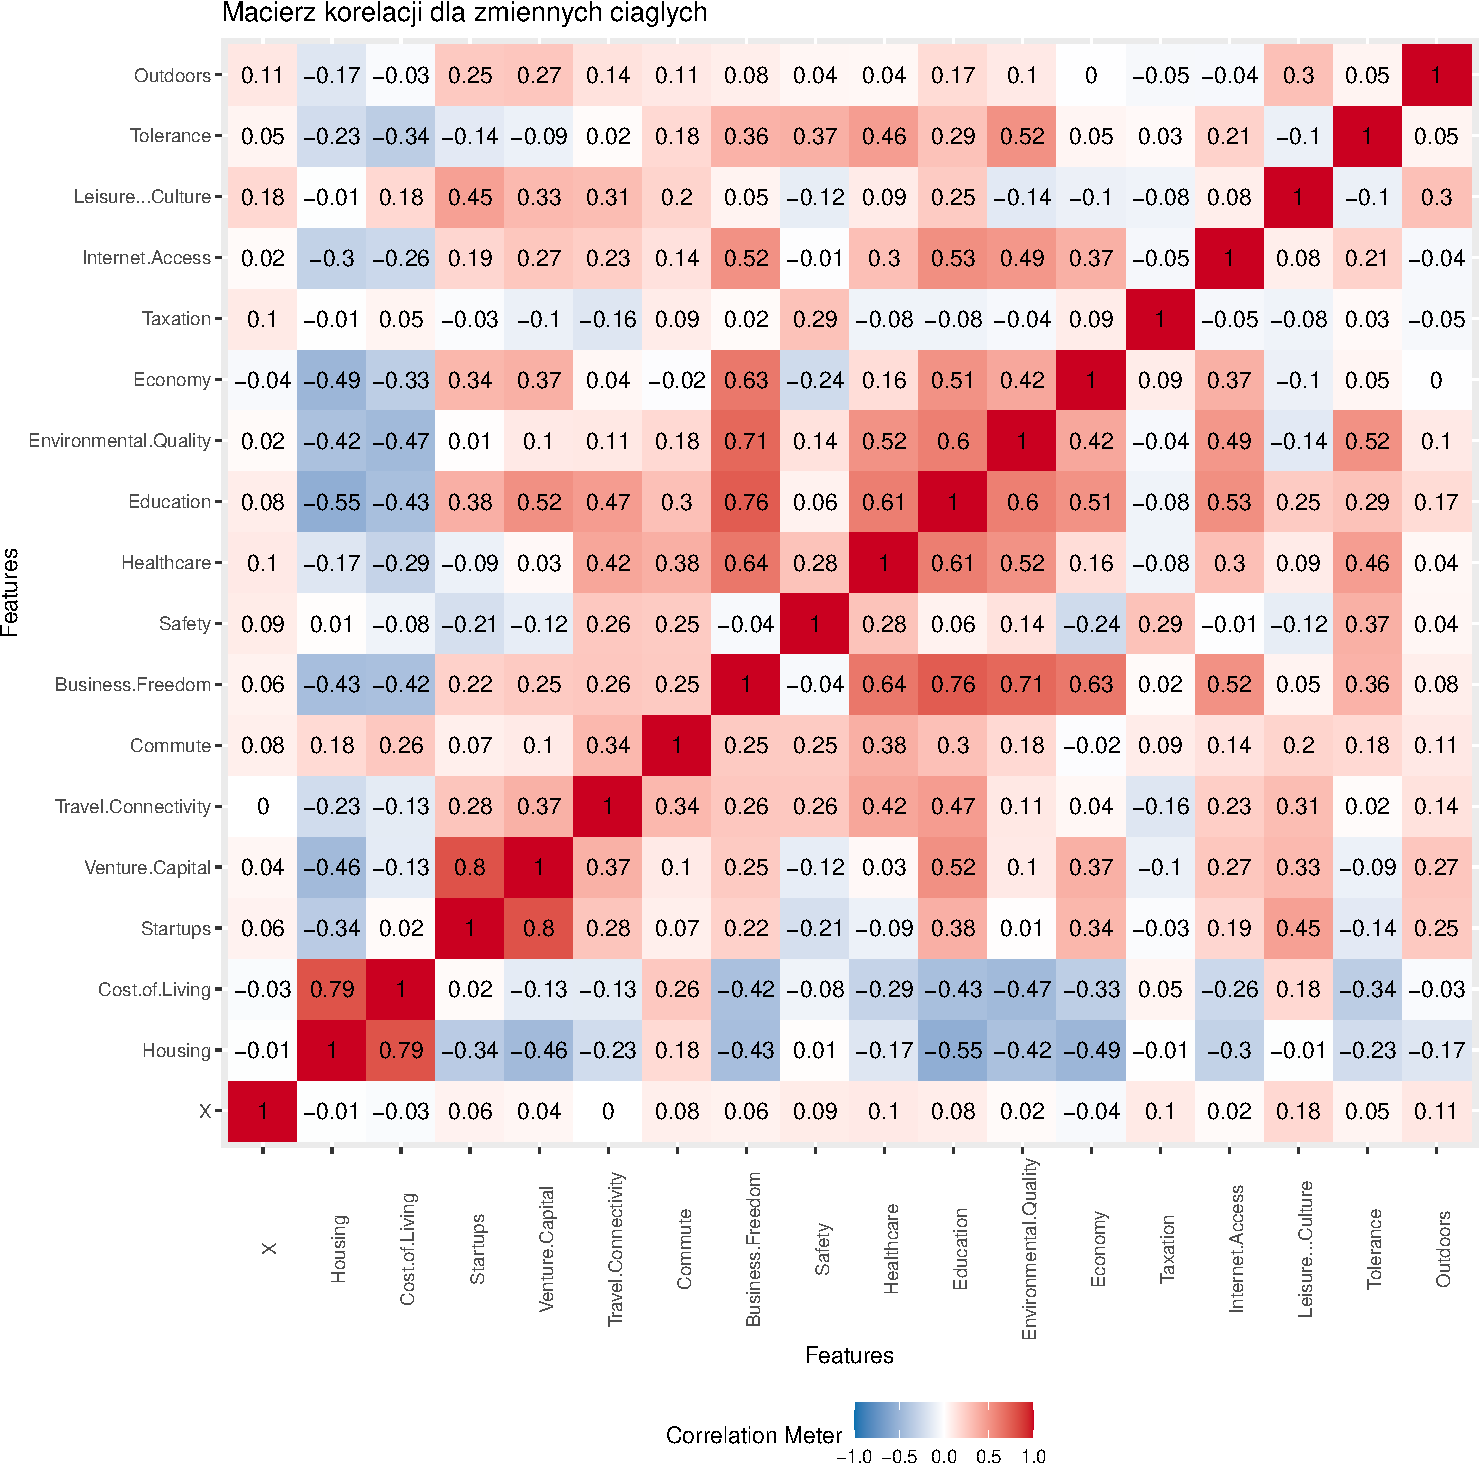
\includegraphics{Sprawozdanie2_files/figure-latex/wykresy_korelacji-1} \end{center}

\begin{center}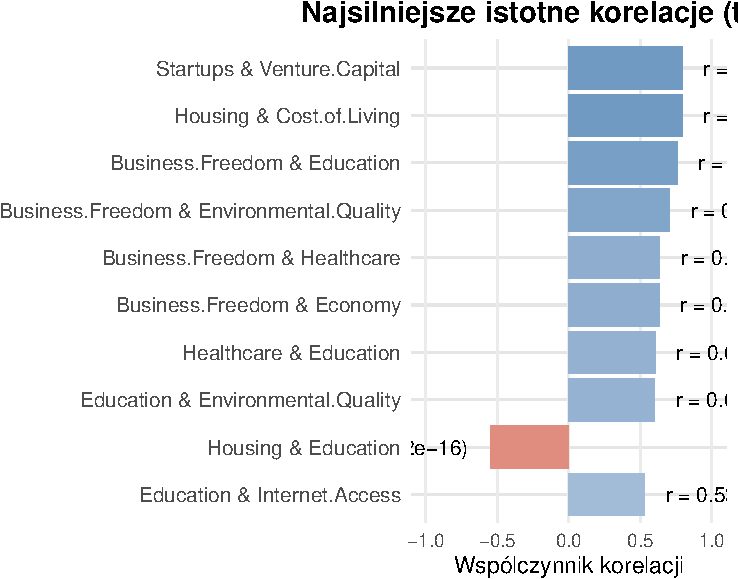
\includegraphics{Sprawozdanie2_files/figure-latex/znaczace_korelacje-1} \end{center}

Z wykresu wynika, że \textbf{najsilniejsza korelacja} występuje między
\textbf{Startups} i \textbf{Venture Capital}, co sugeruje, że dostęp do
kapitału inwestycyjnego silnie wspiera rozwój środowiska startupowego.

Silna zależność widoczna jest również pomiędzy \textbf{Housing} i
\textbf{Cost of Living}, co oznacza, że lepsze warunki mieszkaniowe
często wiążą się z wyższymi kosztami życia.

Silne korelacje dotyczą także:\\
- \textbf{Business Freedom \& Education},\\
- \textbf{Business Freedom \& Environmental Quality},\\
- \textbf{Business Freedom \& Healthcare},\\
- \textbf{Business Freedom \& Economy}

co sugeruje, że \textbf{większa swoboda gospodarcza} często idzie w
parze z \textbf{lepszą edukacją}, \textbf{czystszym środowiskiem},
\textbf{lepszą opieką zdrowotną} i ogólnie \textbf{lepszą gospodarką}.

\begin{longtable}[]{@{}lr@{}}
\toprule\noalign{}
& Wariancja \\
\midrule\noalign{}
\endhead
\bottomrule\noalign{}
\endlastfoot
Housing & 5.265 \\
Cost.of.Living & 5.988 \\
Startups & 4.635 \\
Venture.Capital & 6.520 \\
Travel.Connectivity & 4.375 \\
Commute & 2.320 \\
Business.Freedom & 4.450 \\
Safety & 3.051 \\
Healthcare & 2.196 \\
Education & 4.897 \\
Environmental.Quality & 4.840 \\
Economy & 2.302 \\
Taxation & 2.855 \\
Internet.Access & 3.505 \\
Leisure\ldots Culture & 4.027 \\
Tolerance & 2.974 \\
Outdoors & 2.534 \\
\end{longtable}

\textbf{Dlaczego standaryzacja jest konieczna?}

\begin{itemize}
\tightlist
\item
  Bez standaryzacji \textbf{PCA faworyzuje zmienne} o większym
  zróżnicowaniu, co może prowadzić do \textbf{błędnych wniosków}.
\item
  \textbf{Standaryzacja} (średnia = 0, odchylenie = 1) zapewnia
  \textbf{równomierne traktowanie} wszystkich zmiennych, eliminując
  wpływ \textbf{skali}.
\end{itemize}

\begin{center}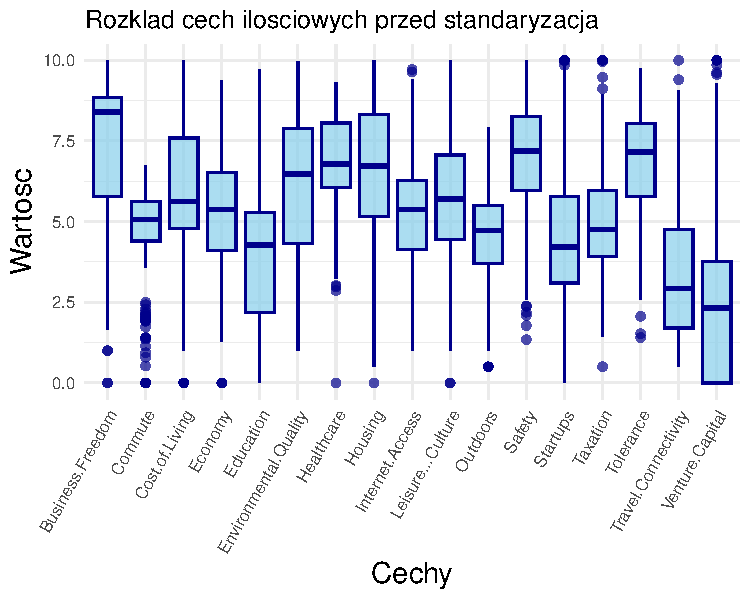
\includegraphics{Sprawozdanie2_files/figure-latex/wykresy_rozkładów_standaryzacja_boxplot-1} \end{center}

\begin{center}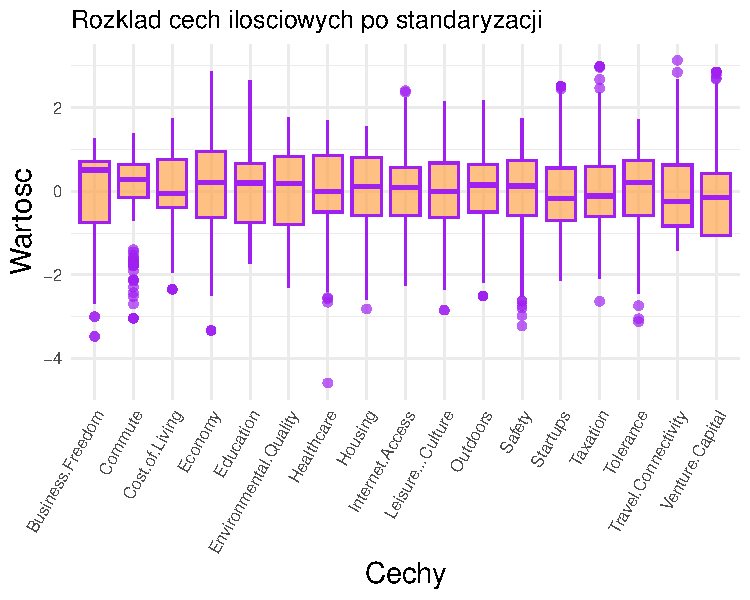
\includegraphics{Sprawozdanie2_files/figure-latex/wykresy_rozkładów_standaryzacja_boxplot-2} \end{center}

\subsection{b) Wyznaczenie składowych
głównych}\label{b-wyznaczenie-skux142adowych-gux142uxf3wnych}

\textbf{Analiza PCA}

\begin{longtable}[]{@{}lrrr@{}}
\toprule\noalign{}
Składowa & Odchylenie\_standardowe & Procent\_wariancji &
Kumulatywna\_wariancja \\
\midrule\noalign{}
\endhead
\bottomrule\noalign{}
\endlastfoot
PC1 & 2.251 & 29.80 & 29.80 \\
PC2 & 1.606 & 15.16 & 44.96 \\
PC3 & 1.443 & 12.25 & 57.21 \\
PC4 & 1.140 & 7.65 & 64.86 \\
PC5 & 1.095 & 7.05 & 71.90 \\
PC6 & 0.980 & 5.65 & 77.55 \\
PC7 & 0.831 & 4.06 & 81.62 \\
PC8 & 0.815 & 3.90 & 85.52 \\
PC9 & 0.764 & 3.43 & 88.95 \\
PC10 & 0.651 & 2.50 & 91.45 \\
PC11 & 0.569 & 1.90 & 93.35 \\
PC12 & 0.539 & 1.71 & 95.06 \\
PC13 & 0.524 & 1.62 & 96.68 \\
PC14 & 0.434 & 1.11 & 97.79 \\
PC15 & 0.393 & 0.91 & 98.69 \\
PC16 & 0.352 & 0.73 & 99.42 \\
PC17 & 0.313 & 0.58 & 100.00 \\
\end{longtable}

\begin{center}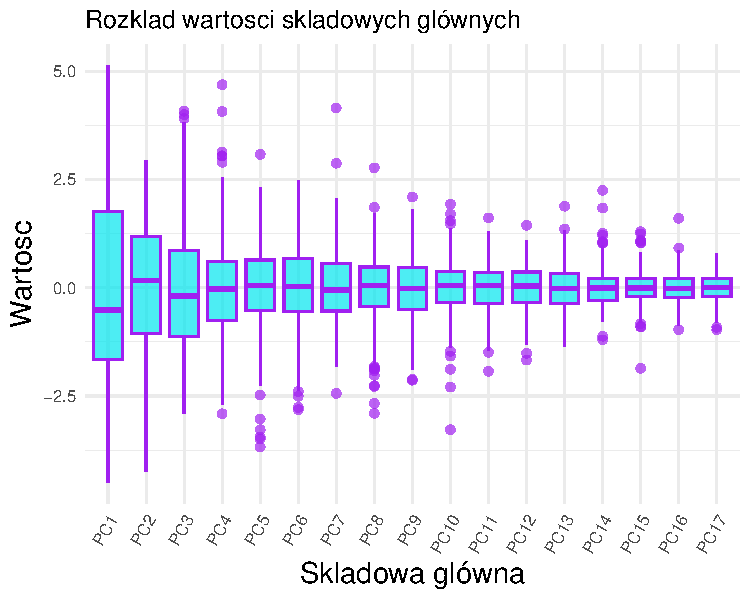
\includegraphics{Sprawozdanie2_files/figure-latex/rozklad_wartosci_wykres_boxplot-1} \end{center}

\textbf{PC1} wykazuje \textbf{największą zmienność}, tłumacząc
największą część wariancji. Kolejne składowe mają coraz mniejszy wpływ
na strukturę danych. Od \textbf{PC7--PC8} zmienność jest
\textbf{niewielka}, co sugeruje ograniczone znaczenie analityczne
dalszych komponentów.

\textbf{Macierz korelacji zmiennych głównych}

\begin{center}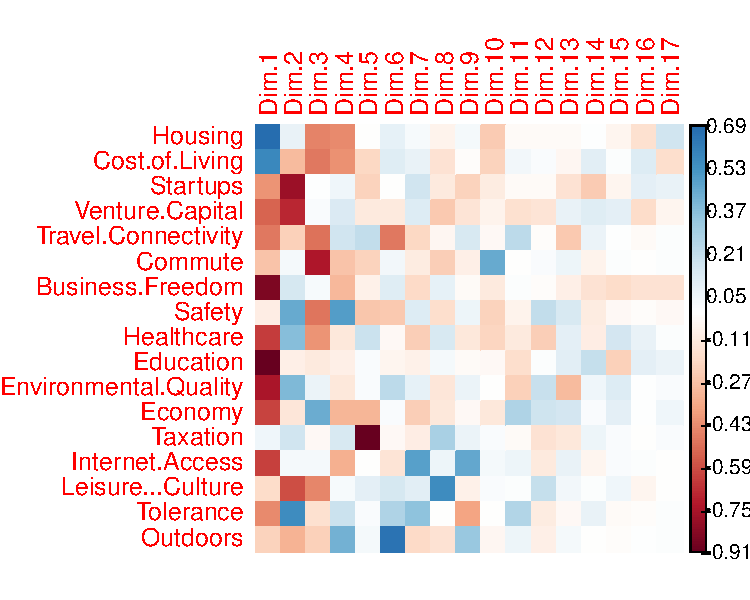
\includegraphics{Sprawozdanie2_files/figure-latex/wykres_istotnosci_zmiennych_w_danych_ladunkach-1} \end{center}

\begin{longtable}[t]{lrrr}
\caption{\label{tab:ladunki}Wektory ładunków dla PC1, PC2 i PC3}\\
\toprule
\cellcolor[HTML]{f2f2f2}{\textbf{}} & \cellcolor[HTML]{f2f2f2}{\textbf{PC1}} & \cellcolor[HTML]{f2f2f2}{\textbf{PC2}} & \cellcolor[HTML]{f2f2f2}{\textbf{PC3}}\\
\midrule
Housing & 0.3078251 & 0.0533534 & -0.3135465\\
Cost.of.Living & 0.2596091 & -0.1757815 & -0.3305352\\
Startups & -0.1802385 & -0.4834415 & 0.0061000\\
Venture.Capital & -0.2365974 & -0.4274509 & 0.0148768\\
Travel.Connectivity & -0.2094543 & -0.1353067 & -0.3397760\\
\addlinespace
Commute & -0.1142045 & 0.0259310 & -0.5057359\\
Business.Freedom & -0.3772809 & 0.0982196 & 0.0241046\\
Safety & -0.0389355 & 0.2871039 & -0.3330100\\
Healthcare & -0.2803590 & 0.2419482 & -0.2810248\\
Education & -0.4025620 & -0.0490795 & -0.0738645\\
\addlinespace
Environmental.Quality & -0.3262220 & 0.2525355 & 0.0535717\\
Economy & -0.2731752 & -0.0740033 & 0.3086705\\
Taxation & 0.0262992 & 0.1074151 & -0.0201849\\
Internet.Access & -0.2761922 & 0.0227056 & 0.0284416\\
Leisure...Culture & -0.0744466 & -0.3647324 & -0.3050545\\
\addlinespace
Tolerance & -0.1897496 & 0.3550911 & -0.1027251\\
Outdoors & -0.0915866 & -0.1933825 & -0.1485868\\
\bottomrule
\end{longtable}

\textbf{Składowa główna 1 (PC1): Jakość życia vs.~dostępność
ekonomiczna}\\
PC1 kontrastuje miasta o wysokiej jakości usług z miastami ekonomicznie
dostępnymi. Najsilniejsze ładunki:

\begin{itemize}
\tightlist
\item
  \textbf{Edukacja} (-0.40),\\
\item
  \textbf{Wolność biznesowa} (-0.38),\\
\item
  \textbf{Jakość środowiska} (-0.33) - wszystkie \textbf{ujemne}\\
\item
  \textbf{Mieszkalnictwo} (0.31),\\
\item
  \textbf{Koszty życia} (0.26) - \textbf{dodatnie}
\end{itemize}

Wysokie wartości PC1 wskazują na miasta o niższych kosztach życia, ale
słabszej infrastrukturze społecznej. Niskie wartości PC1 charakteryzują
rozwiniętą infrastrukturę społeczną przy wyższych kosztach.

\begin{center}\rule{0.5\linewidth}{0.5pt}\end{center}

\textbf{Składowa główna 2 (PC2): Środowisko startupowe vs.~jakość
społeczna}\\
PC2 przeciwstawia ośrodki technologiczne miastom o wysokich wskaźnikach
społecznych:

\begin{itemize}
\tightlist
\item
  \textbf{Startupy} (-0.48),\\
\item
  \textbf{Kapitał venture} (-0.43),\\
\item
  \textbf{Kultura i rozrywka} (-0.36) - \textbf{ujemne}\\
\item
  \textbf{Tolerancja} (0.36),\\
\item
  \textbf{Jakość środowiska} (0.25),\\
\item
  \textbf{Bezpieczeństwo} (0.29) - \textbf{dodatnie}
\end{itemize}

Wysokie wartości PC2 oznaczają miasta bardziej przyjazne społecznie,
niskie wartości wskazują na dynamiczne centra technologiczne.

\begin{center}\rule{0.5\linewidth}{0.5pt}\end{center}

\textbf{Składowa główna 3 (PC3): Komfort codziennego życia
vs.~gospodarka}\\
PC3 zestawia komfort życia codziennego z rozwojem ekonomicznym:

\begin{itemize}
\tightlist
\item
  \textbf{Dojazdy} (-0.51),\\
\item
  \textbf{Połączenia komunikacyjne} (-0.34),\\
\item
  \textbf{Bezpieczeństwo} (-0.33) - \textbf{ujemne}\\
\item
  \textbf{Gospodarka} (0.31) - \textbf{dodatnie}
\end{itemize}

Miasta o wysokich wartościach PC3 mają silną gospodarkę kosztem wygody
życia codziennego, podczas gdy niskie wartości PC3 wskazują na większy
komfort przy mniej dynamicznej ekonomii.

\begin{center}\rule{0.5\linewidth}{0.5pt}\end{center}

\textbf{Podsumowanie}\\
Te trzy wymiary tworzą kompleksowe ramy do klasyfikacji miast:

\begin{itemize}
\tightlist
\item
  \textbf{PC1}: Balans między rozwojem społecznym a dostępnością
  ekonomiczną\\
\item
  \textbf{PC2}: Równowaga między ekosystemem startupowym a jakością
  życia społecznego\\
\item
  \textbf{PC3}: Kompromis między codziennym komfortem a silną gospodarką
\end{itemize}

\subsection{c) Zmienność odpowiadająca poszczególnym
składowym}\label{c-zmiennoux15bux107-odpowiadajux105ca-poszczeguxf3lnym-skux142adowym}

\begin{center}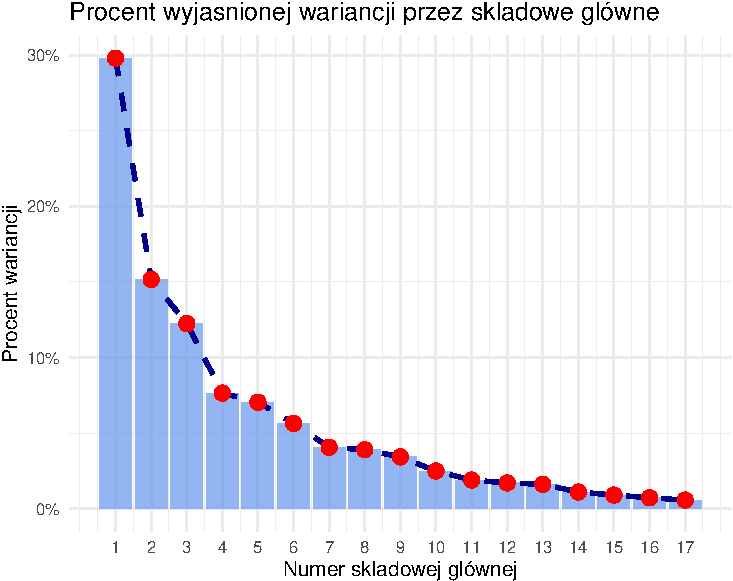
\includegraphics{Sprawozdanie2_files/figure-latex/Zmiennosc_skladowych_w_PCA-1} \end{center}

\begin{center}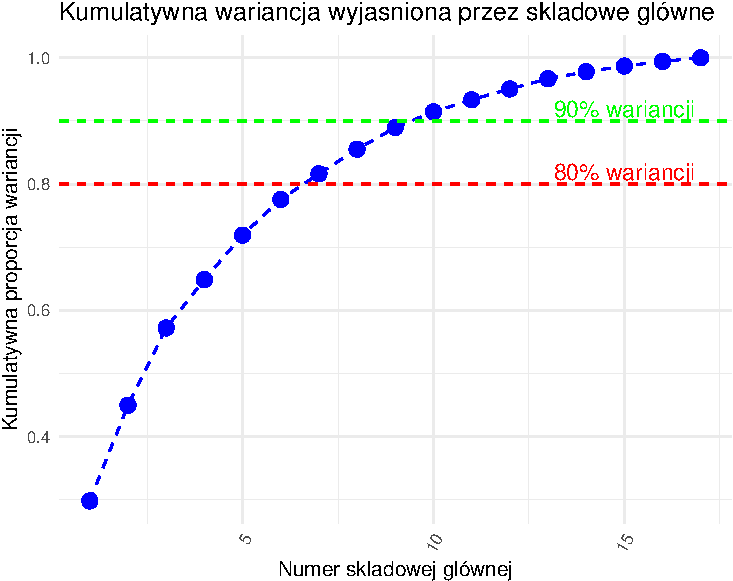
\includegraphics{Sprawozdanie2_files/figure-latex/Zmiennosc_skladowych_w_PCA-2} \end{center}

Na podstawie przedstawionych wykresów można zauważyć, że
\textbf{pierwsze składowe główne} mają największy wpływ na wyjaśnienie
wariancji danych. W szczególności \textbf{pierwsza składowa (PC1)}.
Kolejne składowe, takie jak \textbf{PC2} i \textbf{PC3}, również wnoszą
istotne informacje, ale ich udział w wyjaśnieniu wariancji jest
stopniowo coraz mniejszy.

Z wykresu skumulowanej wariancji można wywnioskować, że pierwsze
\textbf{7} składowych wyjaśnia około \textbf{80\%} całkowitej
zmienności, a pierwsze \textbf{10} składowych odpowiada za \textbf{90\%}
wariancji, co sugeruje, że można ograniczyć liczbę analizowanych cech
bez znaczącej utraty informacji.

\subsection{d) Wizualizacja danych
wielowymiarowych}\label{d-wizualizacja-danych-wielowymiarowych}

\begin{center}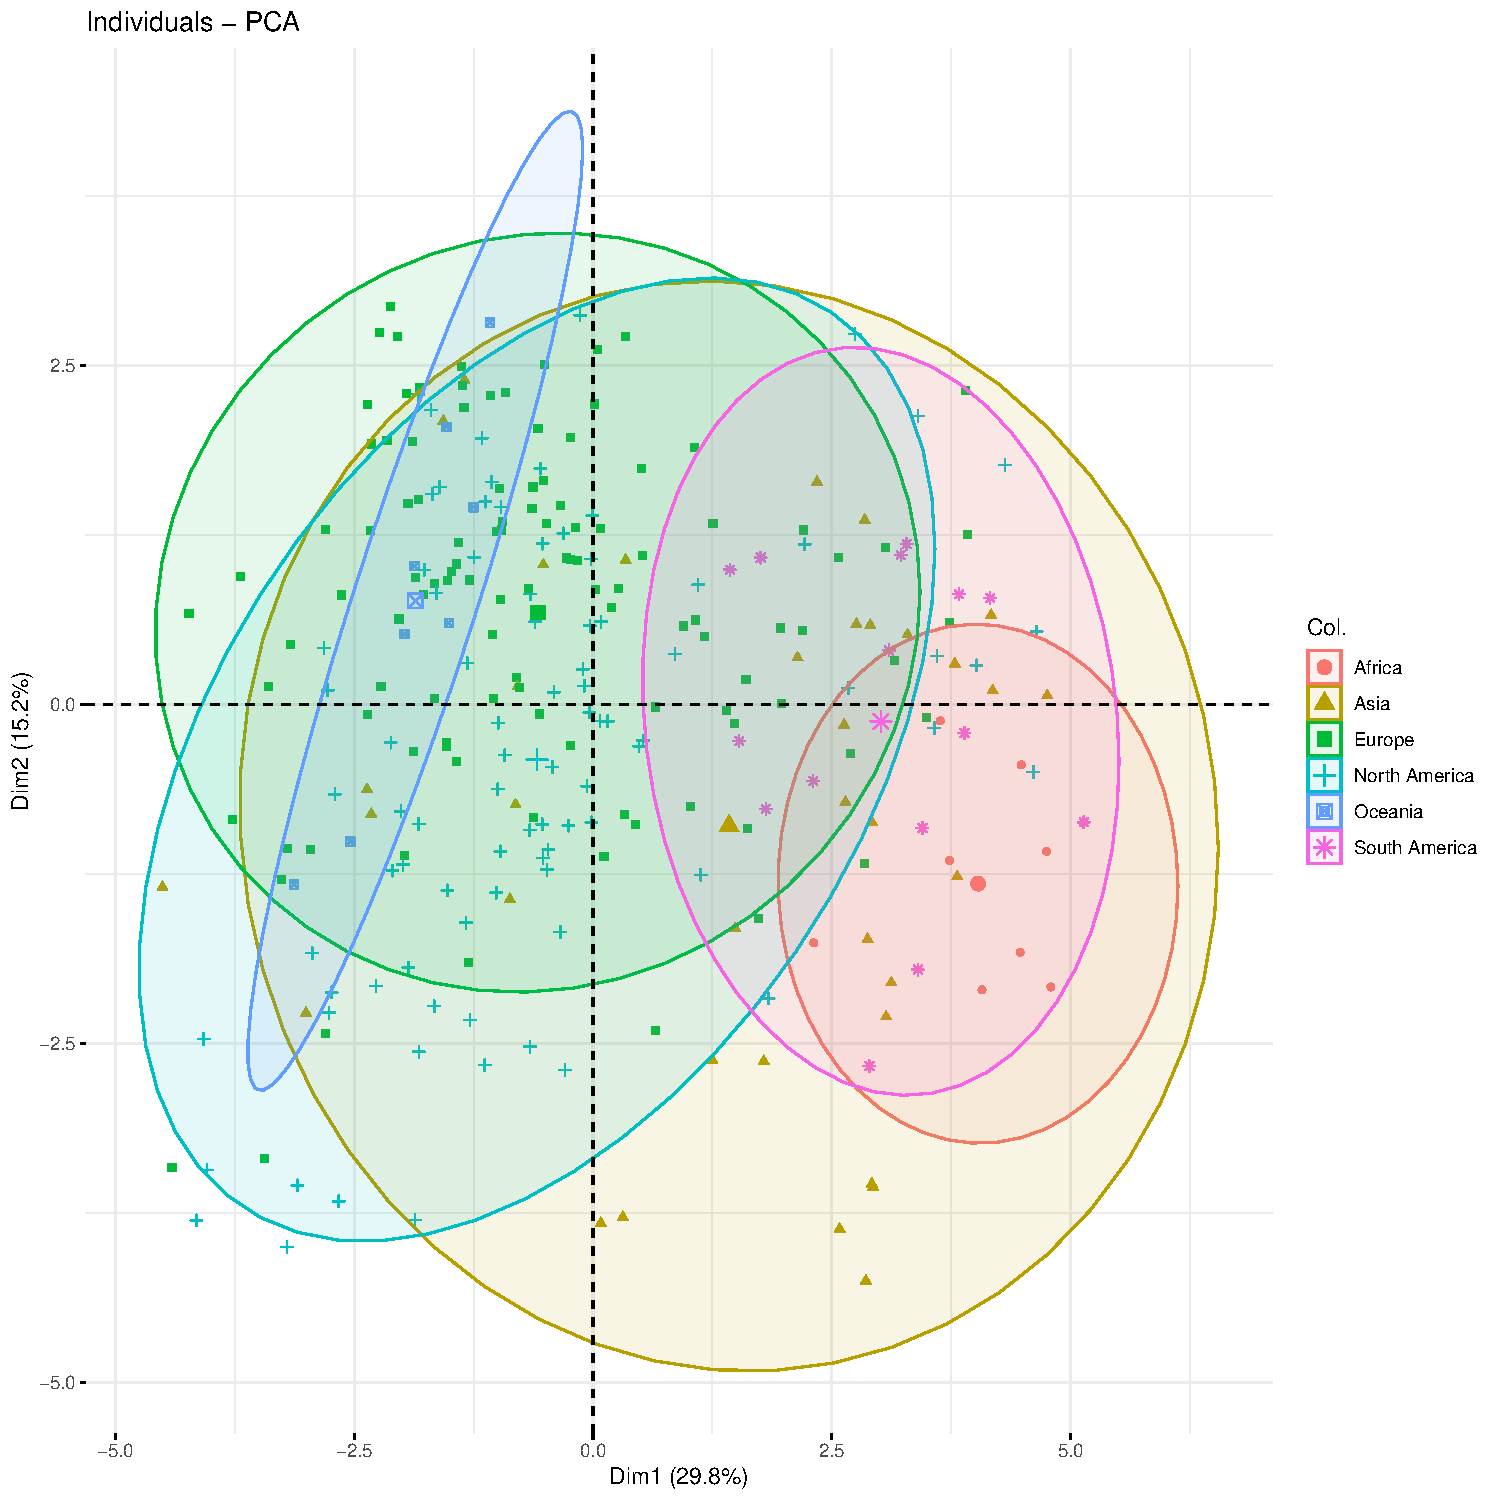
\includegraphics{Sprawozdanie2_files/figure-latex/wykres_2D-1} \end{center}

\textbf{Europa} \emph{(zielone kwadraty)}\\
- Po \textbf{lewej stronie PC1} → \textbf{wysoka jakość życia}, silna
infrastruktura społeczna (edukacja, bezpieczeństwo, środowisko).\\
- \textbf{Wyższe koszty życia}, \textbf{mniejsza dostępność
ekonomiczna}.\\
- Oś PC2 lekko dodatnia → \textbf{zrównoważony rozwój
społeczno-startupowy}.

\textbf{Ameryka Północna} \emph{(turkusowe plusy)}\\
- Również \textbf{lewa strona PC1} → wysoka jakość życia.\\
- \textbf{Niższe wartości PC2} → \textbf{dynamiczne środowisko
technologiczne}, kosztem aspektów społecznych.\\
- Duże \textbf{zróżnicowanie} -- od wybitnie startupowych miast (np.
USA) po umiarkowane.

\textbf{Azja} \emph{(żółte trójkąty)}\\
- \textbf{Niskie koszty życia}, ale \textbf{słabsza jakość usług
społecznych}.\\
- \textbf{Silna obecność centrów startupowych} (np. Singapur, Chiny).

\textbf{Afryka} \emph{(czerwone koła)}\\
- \textbf{Wysokie PC1} → \textbf{niska jakość usług społecznych}, ale
\textbf{dobra dostępność ekonomiczna}.\\
- \textbf{PC2 bliskie zeru} → przeciętna jakość społeczna, \textbf{słabe
środowisko innowacyjne}.

\textbf{Oceania} \emph{(niebieskie romby)}\\
- \textbf{Lewa górna ćwiartka} (PC1 ujemny, PC2 dodatni):\\
- \textbf{Bardzo wysoka jakość życia}, dobre wskaźniki społeczne
(tolerancja, środowisko).\\
- Mało miast, ale \textbf{wyraźnie pozytywne wyniki}.

\textbf{Ameryka Południowa} \emph{(fioletowe gwiazdki)}\\
- \textbf{Blisko środka} (lekko dodatni PC1):\\
- \textbf{Umiarkowana jakość życia}, rozsądne koszty.\\
- \textbf{Niska aktywność startupowa}.

\begin{center}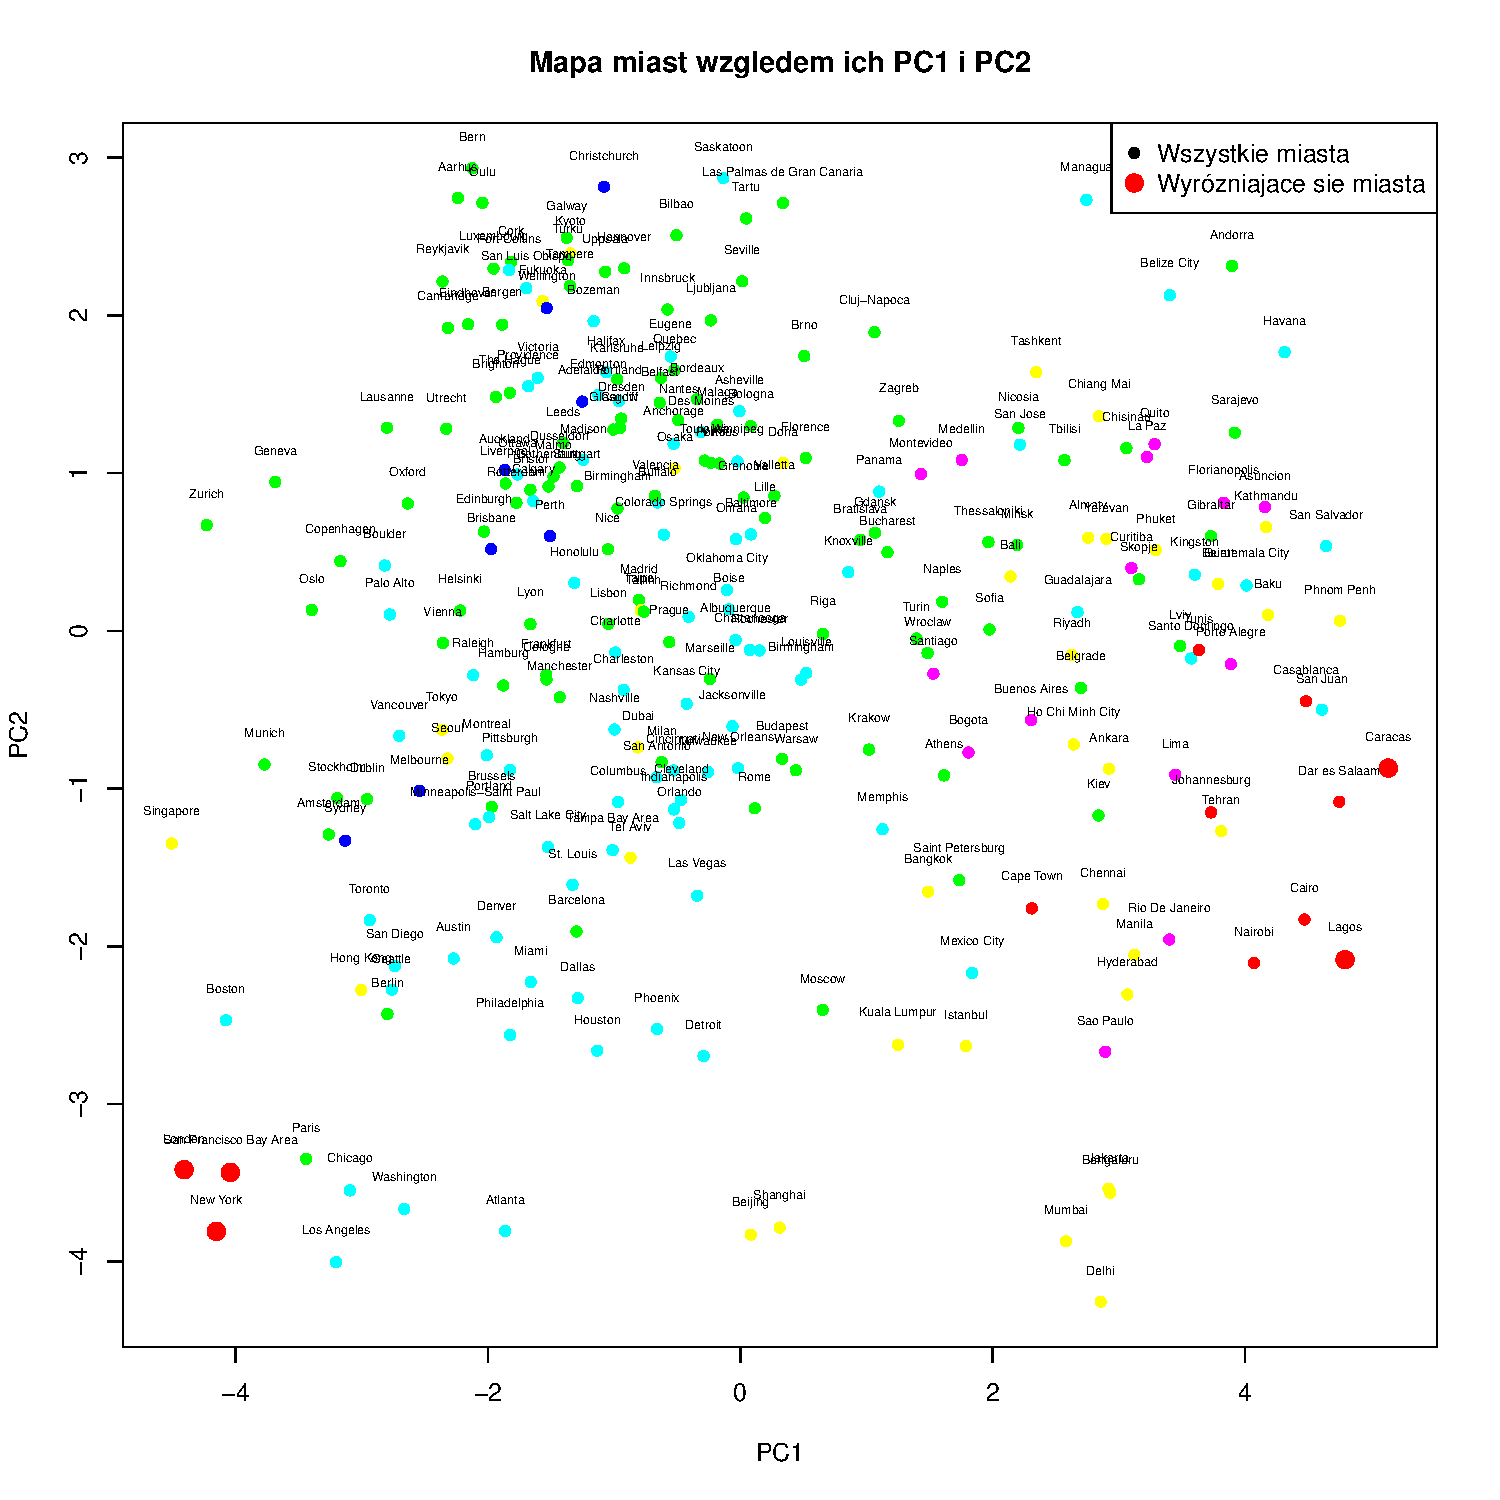
\includegraphics{Sprawozdanie2_files/figure-latex/mapa_wyróżniających_się_miast-1} \end{center}

\begin{longtable}[]{@{}lrrlr@{}}
\caption{Miasta najbardziej oddalone od środka układu współrzędnych
(PCA)}\tabularnewline
\toprule\noalign{}
& PC1 & PC2 & Miasto & Odległość od środka \\
\midrule\noalign{}
\endfirsthead
\toprule\noalign{}
& PC1 & PC2 & Miasto & Odległość od środka \\
\midrule\noalign{}
\endhead
\bottomrule\noalign{}
\endlastfoot
172 & -4.15 & -3.81 & New York & 5.63 \\
139 & -4.41 & -3.42 & London & 5.58 \\
213 & -4.04 & -3.43 & San Francisco Bay Area & 5.30 \\
127 & 4.79 & -2.09 & Lagos & 5.23 \\
53 & 5.14 & -0.87 & Caracas & 5.21 \\
\end{longtable}

\textbf{Miasta najbardziej oddalone od środka układu PCA} charakteryzują
się \textbf{skrajnymi wartościami} dla głównych składowych, co oznacza,
że \textbf{wyróżniają się na tle reszty pod względem profilu jakości
życia, kosztów, rozwoju technologicznego i społecznego}.

\begin{itemize}
\item
  \textbf{Nowy Jork} (\textbf{PC1 = -4.15}, \textbf{PC2 = -3.81}) --
  silnie ujemne wartości obu składowych wskazują na \textbf{wysoką
  jakość infrastruktury społecznej} (PC1) oraz \textbf{intensywnie
  rozwinięte środowisko startupowe} (PC2). To miasto dynamiczne, ale
  jednocześnie \textbf{bardzo kosztowne}.
\item
  \textbf{Londyn} (\textbf{PC1 = -4.41}, \textbf{PC2 = -3.42}) --
  podobnie jak Nowy Jork, łączy \textbf{drogie życie z zaawansowaną
  infrastrukturą społeczną} i \textbf{wysokim rozwojem technologicznym}.
\item
  \textbf{San Francisco Bay Area} (\textbf{PC1 = -4.04}, \textbf{PC2 =
  -3.43}) -- silne centrum technologiczne o \textbf{niskiej dostępności
  ekonomicznej}, ale z \textbf{najwyższą koncentracją startupów i
  kapitału venture}.
\item
  \textbf{Lagos} (\textbf{PC1 = 4.79}, \textbf{PC2 = -2.09}) --
  \textbf{wysoka wartość PC1} oznacza \textbf{niski koszt życia i
  ograniczoną infrastrukturę społeczną}, przy jednoczesnym
  \textbf{udziale w środowisku startupowym} (ujemne PC2). To przykład
  miasta rozwijającego się, ale jeszcze bez zaplecza społecznego.
\item
  \textbf{Caracas} (\textbf{PC1 = 5.14}, \textbf{PC2 = -0.87}) -- miasto
  o \textbf{niskiej jakości życia społecznego} i \textbf{dużej
  ekonomicznej dostępności}, z \textbf{niewielkim zaangażowaniem w
  nowoczesne sektory gospodarki}.
\end{itemize}

\begin{center}\rule{0.5\linewidth}{0.5pt}\end{center}

Te wyniki pokazują, że największe odległości od środka PCA mają zarówno
\textbf{najbardziej rozwinięte miasta świata}, jak i \textbf{najbardziej
marginalne} -- ale \textbf{z różnych powodów}: jedne z powodu
\textbf{nadmiaru infrastruktury i kosztów}, inne z powodu \textbf{braku
zasobów społecznych} i \textbf{niskich kosztów życia}.

\subsection{e) Korelacja zmiennych}\label{e-korelacja-zmiennych}

\begin{center}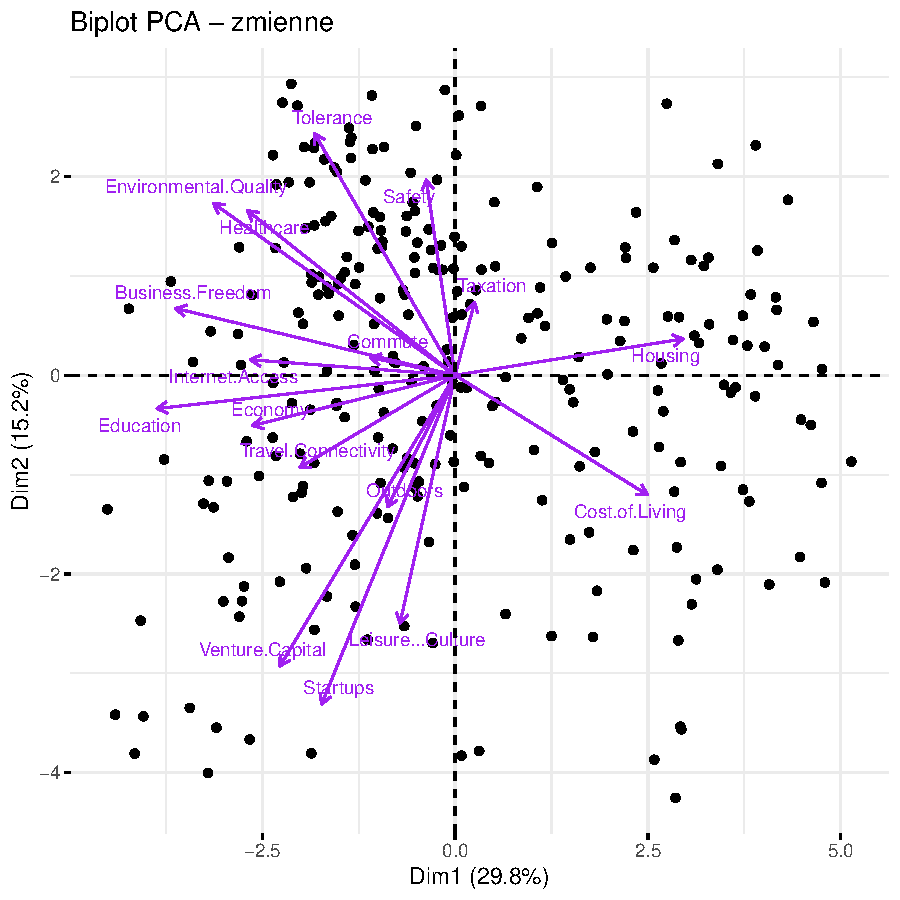
\includegraphics{Sprawozdanie2_files/figure-latex/biplot_koniec-1} \end{center}

\subsubsection{Wnioski z biplotu:}\label{wnioski-z-biplotu}

\begin{itemize}
\tightlist
\item
  \textbf{Długość strzałki} oznacza wpływ zmiennej na PC1 i PC2
\item
  \textbf{Kierunek strzałek}:

  \begin{itemize}
  \tightlist
  \item
    \emph{Zbieżne} → \textbf{dodatnia korelacja}\\
  \item
    \emph{Przeciwne} → \textbf{ujemna korelacja}\\
  \item
    \emph{Prostopadłe} → \textbf{brak korelacji}
  \end{itemize}
\end{itemize}

\paragraph{\texorpdfstring{\textbf{Silne
zależności:}}{Silne zależności:}}\label{silne-zaleux17cnoux15bci}

\textbf{Dodatnie:} - \textbf{Startups -- Venture Capital -- Leisure \&
Culture}\\
- \textbf{Safety -- Tolerance}\\
- \textbf{Business.Freedom - Education - Environmental.Quality}

\textbf{Ujemne:} - \textbf{Cost of Living} vs \textbf{Environmental
Quality}, \textbf{Education}, \textbf{Business Freedom}\\
- \textbf{Housing} vs \textbf{Education}

\textbf{Brak istotnej korelacji:} - \textbf{Safety -- Housing}\\
- \textbf{Commute -- Venture Capital}

\paragraph{Porównanie z macierzą
korelacji:}\label{poruxf3wnanie-z-macierzux105-korelacji}

Wyniki biplotu są spójne z macierzą \texttt{cor()}:

\begin{itemize}
\tightlist
\item
  \textbf{Najsilniejsza korelacja}: \textbf{Startups -- Venture
  Capital}\\
\item
  \textbf{Housing -- Cost of Living}\\
\item
  \textbf{Housing - Education}
\item
  \textbf{Business Freedom} silnie koreluje z:

  \begin{itemize}
  \tightlist
  \item
    \textbf{Education}
  \item
    \textbf{Environmental Quality}
  \item
    \textbf{Healthcare}
  \item
    \textbf{Economy}
  \end{itemize}
\end{itemize}

\subsection{f) Końcowe wnioski}\label{f-koux144cowe-wnioski}

Na podstawie przeprowadzonych analiz i wyników biplotu, kilka istotnych
wniosków:

\begin{enumerate}
\def\labelenumi{\arabic{enumi}.}
\tightlist
\item
  \textbf{Reprezentacja danych}:

  \begin{itemize}
  \tightlist
  \item
    \textbf{PC1} i \textbf{PC2} wyjaśniają główną część zmienności
    danych, szczególnie \textbf{PC1}, która tłumaczy różnice w jakości
    życia i dostępności ekonomicznej. \textbf{PC3} dostarcza dodatkowych
    informacji, ale ma mniejszy wpływ. Pierwsze 2--3 składowe wyjaśniają
    około \textbf{80\% wariancji}.
  \end{itemize}
\item
  \textbf{Składowe główne}:

  \begin{itemize}
  \tightlist
  \item
    \textbf{PC1} (Jakość życia vs.~dostępność ekonomiczna): Większość
    miast znajduje się na przeciwnych końcach tej osi, pokazując różnice
    w równowadze między wysokimi kosztami życia a rozwiniętą
    infrastrukturą społeczną.
  \item
    \textbf{PC2} (Środowisko startupowe vs.~jakość społeczna): Składa
    się z zmiennych takich jak ``Startups'', ``Venture Capital'' i
    ``Leisure \& Culture'', które opisują dynamiczne ośrodki
    technologiczne.
  \item
    \textbf{PC3} (Komfort życia vs.~gospodarka): Zestawia miasta o
    silnej gospodarce z tymi, które oferują wyższy komfort życia
    codziennego.
  \end{itemize}
\item
  \textbf{Znaczenie standaryzacji}:

  \begin{itemize}
  \tightlist
  \item
    \textbf{Standaryzacja} zmiennych miała kluczowy wpływ na wyniki PCA.
    Bez niej, zmienne o większym zróżnicowaniu (np. koszty życia)
    mogłyby dominować, prowadząc do błędnych wniosków. Po standaryzacji,
    każda zmienna ma równy wpływ, co zapewnia bardziej sprawiedliwą
    ocenę.
  \end{itemize}
\item
  \textbf{Geograficzne różnice}:

  \begin{itemize}
  \tightlist
  \item
    Z analizy biplotu wynika, że miasta rozmieszczone są zgodnie z
    globalnymi różnicami w jakości życia, dostępności ekonomicznej i
    rozwoju startupów. Duże zróżnicowanie występuje między miastami
    rozwiniętymi (np. Nowy Jork, Londyn) a tymi na początku drogi
    rozwoju (np. Lagos, Caracas). Wiele miast z krajów rozwiniętych
    znajduje się w lewym dolnym rogu biplotu, co wskazuje na
    \textbf{wysoką jakość usług społecznych} i \textbf{wyższe koszty
    życia}.
  \end{itemize}
\end{enumerate}

\subsubsection{Wnioski ogólne:}\label{wnioski-oguxf3lne}

\begin{itemize}
\tightlist
\item
  \textbf{Analiza PCA} dostarcza cennych informacji o relacjach między
  różnymi aspektami życia w miastach. Widać, że miasta o wyższych
  kosztach życia mają rozwiniętą infrastrukturę społeczną, podczas gdy
  te o niższych kosztach życia oferują mniejszy rozwój infrastruktury,
  ale większy dostęp do rozwoju gospodarczego.
\item
  \textbf{Standaryzacja} jest kluczowa do uzyskania rzetelnych wyników
  PCA, eliminując wpływ różnic w skali danych.
\end{itemize}

\section{ZADANIE 3 (Skalowaniewielowymiarowe (Multidimensional Scaling
(MDS)))}\label{zadanie-3-skalowaniewielowymiarowe-multidimensional-scaling-mds}

\subsection{a) Dane: titanic\_train (R-pakiet
titanic)}\label{a-dane-titanic_train-r-pakiet-titanic}

Zbiór danych zawiera wybrane charakterystyki opisujące pasażerów
Titanica (w tym m.in. takie zmienne jak: wiek, płeć, miejsce rozpoczęcia
podróży czy klasa pasażerska) wraz z informacją czy dana osoba przeżyła
katastrofę (zmienna Survived).

\subsection{b) Przygotowanie danych}\label{b-przygotowanie-danych}

Wczytane dane, niepotrzebne kolumny zostały usunięte, oraz typy
poszczególnych cech zostały zaaktualizowane na odpowiednie czyt.
ordered,numeric

\subsection{c) Redukcja wymiaru na bazie
MDS}\label{c-redukcja-wymiaru-na-bazie-mds}

Redukuję wymiar danych korzystając z \textbf{metody metrycznej (Funkcja
cmdscale)}

Kolejno tworzymy diagram Shepherda

\begin{center}\includegraphics{Sprawozdanie2_files/figure-latex/diagram shepherda-1} \end{center}

\textbf{Ocena jakości odwzorowania -- Diagram Shepherda}

Na powyższym wykresie porównano oryginalne odległości (metoda Gowera) z
odległościami otrzymanymi po zastosowaniu MDS.

\textbf{Większość punktów układa się wzdłuż linii x = y}, co wskazuje na
dobre odwzorowanie struktury danych. Choć niektóre punkty od niej
odbiegają, to \textbf{różnice są stosunkowo niewielkie} -- zwłaszcza w
zakresie mniejszych odległości, które są najbardziej istotne dla
zachowania lokalnej struktury danych.

\textbf{Wniosek:} Transformacja MDS zachowała strukturę danych na
akceptowalnym poziomie. Diagram Shepherda potwierdza, że skalowanie
wielowymiarowe wiernie odtworzyło relacje między punktami, szczególnie w
przypadku najbliższych sąsiadów.

\subsection{d) Wizualizacja danych}\label{d-wizualizacja-danych}

\begin{center}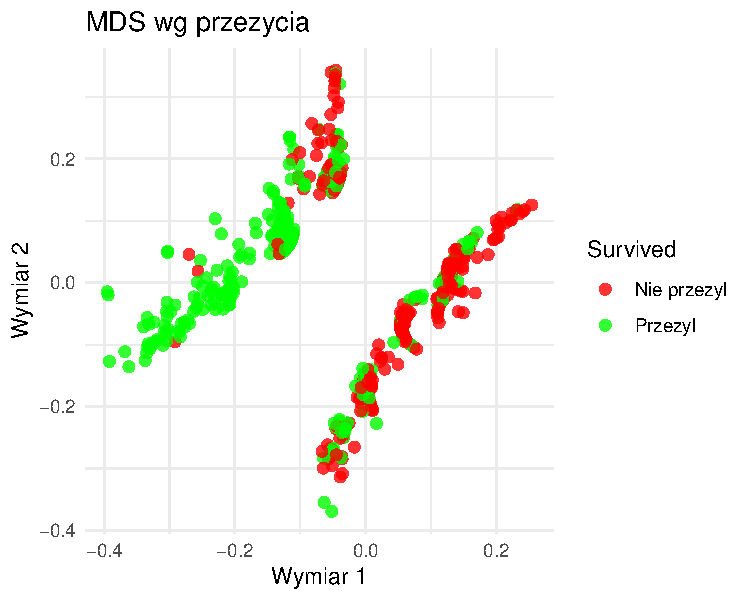
\includegraphics{Sprawozdanie2_files/figure-latex/rozrzut 2D-1} \end{center}

Na powyższym wykresie przedstawiono wynik analizy MDS, w której obiekty
zostały rozróżnione ze względu na zmienną \texttt{Survived}.

Na wykresie wyraźnie widoczny jest \textbf{podział obiektów na dwa
skupiska}. Pierwsze z nich (po lewej stronie wykresu) charakteryzuje się
\textbf{dużym odsetkiem osób, które przeżyły}, natomiast drugie (po
prawej) skupia głównie osoby, które \textbf{nie przeżyły}.

Nie zaobserwowano \textbf{obserwacji odstających} ani punktów
jednoznacznie nietypowych --- wszystkie dane mieszczą się w obrębie
naturalnych skupisk.

Na podstawie wykresu można wnioskować, że \textbf{analiza MDS skutecznie
wydobyła ukrytą strukturę danych}, związaną ze zmienną
\texttt{Survived}.

\begin{center}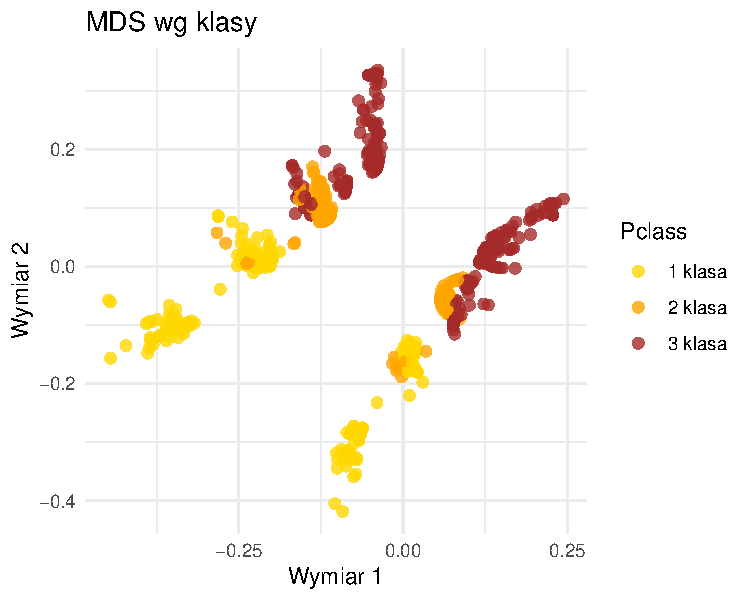
\includegraphics{Sprawozdanie2_files/figure-latex/wyk2-1} \end{center}

Na powyższym wykresie przedstawiono wynik analizy MDS z uwzględnieniem
klasy, w której podróżowali pasażerowie (\texttt{Pclass}).

Rozkład punktów w przestrzeni odwzorowanej za pomocą MDS jest stosunkowo
\textbf{równomierny}, a poszczególne klasy są \textbf{rozproszone w
obrębie różnych skupisk}. Nie obserwuje się jednoznacznej separacji
przestrzennej ze względu na klasę podróży. Wskazuje to na \textbf{brak
silnej zależności między zmienną \texttt{Pclass} a układem punktów w
przestrzeni MDS}.

W odróżnieniu od zmiennej \texttt{Survived}, która wykazywała wyraźną
strukturę klasową, tutaj nie ma widocznych skupisk odpowiadających
konkretnym klasom. W każdej z trzech głównych grup przestrzennych
występują pasażerowie różnych klas, co sugeruje, że klasa podróży
\textbf{nie była głównym czynnikiem różnicującym obserwacje} w tej
analizie wielowymiarowej.

Nie zaobserwowano również punktów odstających ani obserwacji nietypowych
--- dane układają się w sposób naturalny i uporządkowany.

\begin{center}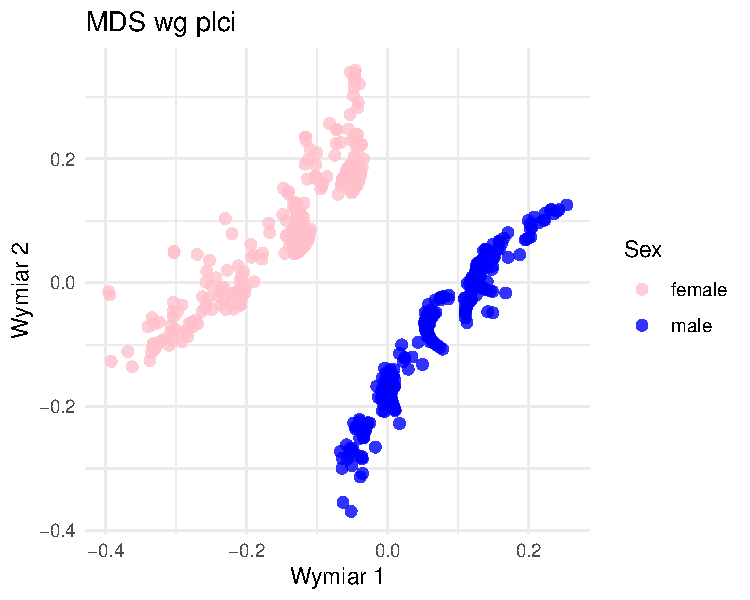
\includegraphics{Sprawozdanie2_files/figure-latex/wyk3-1} \end{center}

Na powyższym wykresie przedstawiono wynik analizy MDS z podziałem na
płeć pasażerów (\texttt{Sex}). Widoczny jest \textbf{wyraźny podział} na
dwie grupy, odpowiadające kobietom i mężczyznom.

Porównując ten wykres z wcześniejszą analizą przeżywalności
(\texttt{Survived}), można zauważyć, że grupa odpowiadająca kobietom
\textbf{częściej pokrywa się} z obszarami o wyższej przeżywalności. Jest
to zgodne zarówno z intuicją, jak i historycznymi danymi dotyczącymi
katastrofy Titanica, gdzie kobiety miały znacznie większe szanse
przeżycia niż mężczyźni.

Podobnie jak wcześniej, \textbf{nie zaobserwowano istotnych obserwacji
odstających}, co świadczy o dobrej jakości danych i prawidłowym
odwzorowaniu relacji między obserwacjami.

\end{document}
